% !TEX root = ../main.tex
\chapter{Post-Supernova Kinematics: The Natal Kick}\label{chap:natal_kicks}

\mediaepigraph{And the memories were lost long ago\\But at least you have beautiful ghosts.}{Beautiful Ghosts}{Taylor Swift}

\lettrine[lines=3]{T}{he terminus of a massive star's} life is a core-collapse supernova, when the hydrostatic equilibrium between the pressure of the star and its self-gravity is broken, and the stellar core collapses in on itself. Once the star reaches nuclear densities, neutron degeneracy is able to stabilise the remnant, causing a shockwave to propagate outwards from the core. The energy released is roughly an order of magnitude greater than the binding energy of the star \citep{Eldridge:2018}, resulting in the ejection of an amount of mass we denote $M_\text{ej}$ and leaving a remnant of mass $M_\text{rem}$ behind. If the ejection is asymmetric, the collapse endows the nascent remnant with a velocity $v_\text{k}$ whose overall direction is antialigned to the more massive ejecta. This motion is termed a natal supernova kick.

Given an observation of the proper velocity of a compact remnant, it is in principle possible to trace its motion back and ascertain its kick velocity. However, this is not necessarily a straightforward endeavour. If the proper velocity is high and the remnant old, it has travelled quite a distance from its explosion site to be located at the point the observation has been taken. In addition, the star has potentially had its proper velocity modified by gravitational attraction from either other runaway stars or its host galaxy's potential. One would require the exact location in 3D space as well as the 3D velocity and remnant age in order to ascertain the motion, but from there the inverse problem becomes straightforward.

\section{Overview}

As a consequence of conservation of momentum, it can be shown that if the ejecta is assumed to eject along a preferred axis, the velocity of the kick can be written as

\begin{equation}
    v_\text{k} = \alpha\left(\frac{M_\text{ej}}{M_\text{rem}}\right)+\beta\left(\frac{M_\text{NS}}{M_\text{rem}}\right),\label{eq:bray_kick_pure}
\end{equation}

for free parameters $\alpha$ and $\beta$ (both measured in $\si{\km\per\second}$). Here, $M_\text{NS}$ is the mass of a \gls{ns}; if the kick is applied to a \gls{ns}, then $M_\text{NS}=M_\text{rem}$ and the coefficient reduces to unity. If the kick is applied to a \gls{bh}, then we can take $M_\text{NS}=\SI{1.4}{\msun}$, which serves to convert the distribution from one in velocity-space to one in momentum-space; see \citet{Bray:2016, Bray:2018, Richards:2023} for further detail.

This parameterization introduces, effectively, four free parameters in $\alpha, \beta, \theta, \phi$ (the latter two being azimuthal and equatorial angles of the ejecta mass). We assume that the preferential axis is sampled uniformly across the $4\pi$ steradians of the star, and that our only two free parameters are $\alpha$ and $\beta$. It is pertinent to note two things due to this assumption: firstly, we are not assuming that the ejection occurs along one axis and that the kick is aligned along a different, random, axis. Rather, we are assuming that the asymmetric ejection occurs along a randomly sampled axis and that the kick is antialigned to that. The second note, explored further in \autoref{sec:natal_kick_prescriptions}, is that there is considerable uncertainty around the nature of the kick and the precise mechanism that causes it to eject along a given axis. This is the reason we sample the kick direction uniformly, though we will simulate sufficiently many systems (on the order of $\mathcal{O}(10^{12})$) that this will be marginalised over.

The existence of two free parameters, $\alpha$ and $\beta$, mean that a choice on the values must be made. The ``traditional'' way to choose these parameters, as outlined in \citet{Bray:2016, Bray:2018}, is to refine them based on isolated pulsar velocities. This methodology, however, has significant drawbacks. Notably, the reliance on one observation can engender biases in the result at the expense of no longer predicting accurate results for other observables. For instance, in the limit of \glspl{ussne} where the ejecta-remnant mass ratio becomes small, the fiducial kick in \citet{Bray:2018} would produce kick velocities that are strongly negative (indicating a strong kick aligned with the direction of motion of the ejecta), contrasted with the weak kicks we expect from these supernovae \citep[e.g.,][]{Willcox:2021}. It becomes evident that a new series of empirical tests are needed, whereupon more constraints than simply pulsar velocities are tested. In this Chapter, we outline four such tests that form the basis of the work of \citet{Richards:2023}. These tests -- using observed \gls{lvk} merger rates, period-eccentricity distributions of \glspl{bns}, isolated pulsar velocities, and production of \glspl{ussne} -- allow us to narrow the parameter space significantly, with the promise of future refinement with more observations (such as through \gls{lvk} \gls{o4}).

\subsection{Parameter space}

We perform our computation on three populations, termed \textsc{FineGrid}, \textsc{WideGrid}, and \textsc{Hobbs}, whose properties are outlined in \autoref{tab:populations}. These populations simulate 1,000 kicks per system sampled. The aim of the three populations is twofold. Firstly, by generating \textsc{FineGrid} and \textsc{WideGrid}, we are able to look both at fine detail in the region at which the most likely value is expected to lie and also the large-scale behaviour over wider parameter ranges.

\begin{table}[h]
    \centering

    \begin{tabular}{l|cc|cc|c}
        \toprule
        \textbf{Population Name} & $\alpha_\text{low}$ [\unit{\km\per\s}] & $\alpha_\text{high}$ [\unit{\km\per\s}] & $\beta_\text{low}$ [\unit{\km\per\s}] & $\beta_\text{high}$ [\unit{\km\per\s}] & Step Size [\unit{\km\per\s}] \\
        \midrule
            \textsc{FineGrid} & 0 & 400 & -200 & 200 & 10 \\
            \textsc{WideGrid} & 0 & 700 & -350 & 350 & 50 \\
            \textsc{Hobbs} & - & - & - & - & - \\
        \bottomrule
    \end{tabular}

    \caption[The populations under study.]{The populations under study. \textsc{Hobbs} is a fiducial kick prescription as given by \citet{Hobbs:2005}, which is a Maxwellian distribution with distribution parameter $\sigma=\SI{265}{\km\per\s}$, based on an empircal fit to the velocities of 233 pulsars. All three prescriptions simulated 1,000 kicks for each system, with the resultant kick being the mean velocity sampled, and the direction of the kick being sampled uniformly across the $4\pi$ steradians of the orbit.}
    \label{tab:populations}
\end{table}

Secondly, by using \citet{Hobbs:2005}, we are able to create a population governed by a kick that has been well-tested in literature \citep[see, for example,][]{Bouffanais:2021, Broekgaarden:2021, Fragione:2021, Igoshev:2021, Mandel:2021} which serves as a fiducial comparison. From a Bayesian perspective, we are essentially choosing the \textsc{Hobbs} distribution as our prior for the express purpose of a Bayesian test in \autoref{sec:per_ecc_dist}.

The choice of extremal values for $\alpha$ and $\beta$ are somewhat arbitrary. \autoref{fig:grid_regions} shows a wider parameter space with $\alpha\in\left[0, 1000\right], \beta\in\left[-500, 500\right]$. Regions in the upper right (bottom left) corner of the plot have quite high (low) mean kick velocities. Although both grids encroach on these regions somewhat, there is a tradeoff between exploring the grid space fully and using computational resources efficiently. Our mean kick velocities should not be too extreme; the mean for a \citet{Hobbs:2005} kick is $\sigma=\SI{265}{\km\per\s}$, for a \citet{Verbunt:2017} is $\sigma_1=\SI{75}{\km\per\s}$ and $\sigma_2=\SI{316}{\km\per\s}$, and for the observed \citet{Willcox:2021} kick $\sigma_1\approx\SI{30}{\km\per\s}, \sigma_2\approx\SI{230}{\km\per\s}$. These\footnote{Due to the grid size and the random sampling, a true contour is difficult to observe due to sampling noise. The contours shown are thus linear fits to the actual contours.} are shown on the grid as black lines.

Whilst the exact parameters can be shifted somewhat and maintain the statistical integrity given these constraints, there are a few additional heuristic constraints we place on the regions to select. First, we wish to capture low-velocity \gls{ussne} kicks (as will be discussed in \autoref{sec:ussne_production}), necessitating a region near $\alpha=\beta=0$ (where the kick would be identically zero for all ejecta-remnant mass ratios). Secondly, the fiducial work of \citet{Bray:2018} found $\alpha=100, \beta=-170$. Although a goal was to (ideally) remove $\beta<0$ as a possible value (for \gls{ussne} again), to impose that as a prior when the fiducial value sat within that range would have gone contrary to typical Bayesian practices. Thirdly, we expected but could not guarantee that the magnitude of each parameter would shrink with further tests, given the large uncertainty bands that \citet{Bray:2018} found (hence broadening our search area beyond $\left|\alpha\right|=100, \left|\beta\right|=170$). Finally, we elected to increase the grid search region by 75 per cent for \textsc{WideGrid} as this would allow us to just reach $\bar{v}_\text{k}=\SI{700}{\km\per\s}$, which is where the \gls{cdf} of the \citet{Hobbs:2005, Verbunt:2017, Willcox:2021} distributions all (approximately) begin to level out (signifying few velocities above those), as shown in \autoref{fig:bray_vs_hobbs_vs_willcox_pdf}.

\begin{figure}[!htbp]
    \centering
    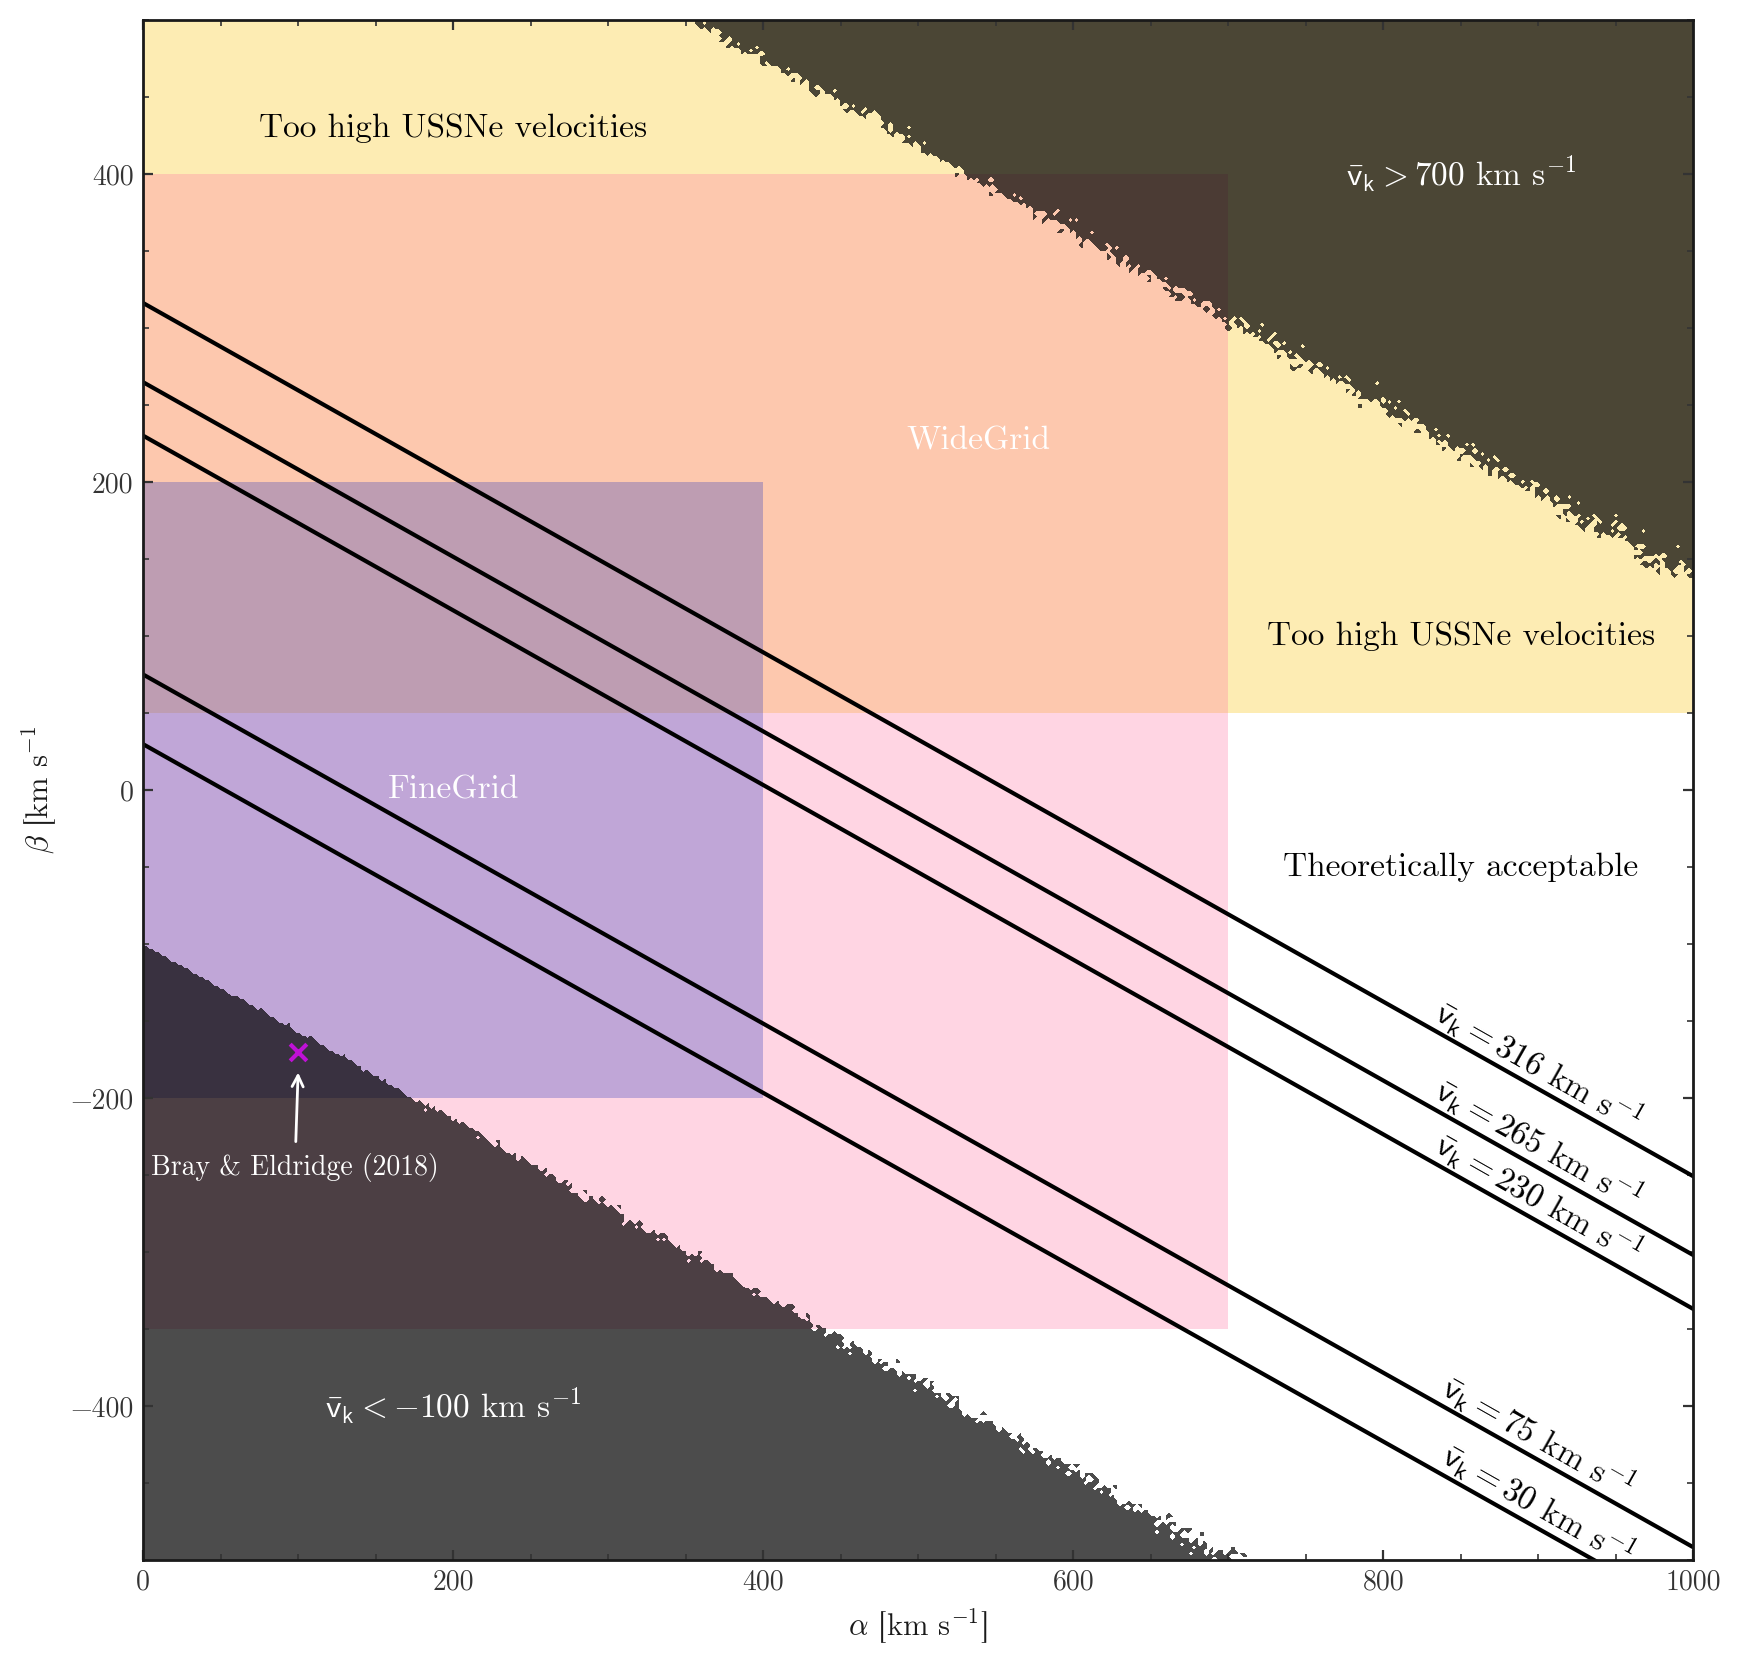
\includegraphics[width=\textwidth]{images/NatalKicks/Grid_Regions.png}
    \caption[A schematic of how \textsc{FineGrid} and \textsc{WideGrid} are related.]{A schematic of how \textsc{FineGrid} and \textsc{WideGrid} are related. The mean kick velocity $v_\text{k}$ was computed by averaging the kick velocities of 1,000 simulated kicks for each combination of $\alpha$ and $\beta$, with $m_\text{rem}\in\left[0.1, 2.5\right]$ and $m_\text{ej}\in\left[0.1, m_\text{rem}\right]$ sampled uniformly. The pink cross represents the point $\alpha=100, \beta=-170$, which are the fiducial kick parameters from \citet{Bray:2018}.}
    \label{fig:grid_regions}
\end{figure}

\subsection{Natal Kick Prescriptions}\label{sec:natal_kick_prescriptions}

There are conflicting accounts as to the cause of the kick \citep[see, for example,][]{Fryer:1998, Arzoumanian:2002, Bombaci:2004, Hobbs:2005, Bray:2016, Verbunt:2017}. There are conflicting accounts as to the form and distribution of the kick too, as discussed in, for example, \citet{Blaauw:1961, Gunn:1970, De_loore:1975, Sutantyo:1978, Hobbs:2005, Baker:2008, Wongwathanarat:2013, Bray:2018, Giacobbo:2020, Mandel:2020}.

We stress that we are not attempting to prescribe \textit{which} prescription is somehow ``best'', but seek an easy-to-configure kick which allows us to configure kicks without changing any of the physics of how our population was formed. This can be done by modifying the kick of \citet{Bray:2016}, which takes two free parameters which can be changed without imposing constraints on physics. This prescription is hereinafter referred to as the ``Bray kick''. Similarly, we require for the purposes of computing log-Likelihoods in \autoref{sec:per_ecc_dist} a comparison kick, for which we select the kick of \citet{Hobbs:2005}, a well-known empirically derived kick. This prescription is hereinafter referred to as the ``Hobbs kick''.

The Bray kick velocity is prescribed by \autoref{eq:bray_kick_pure}. The coefficient to the $\beta$ term, $\frac{M_\text{NS}}{M_\text{rem}}$, serves to generalise the kick from purely \glspl{ns} to \glspl{bh} as well. When applied to a \gls{bh}, $M_\text{NS}$ is taken to be \SI{1.4}{\msun}, and conversely when applied to a \gls{ns}, $M_\text{NS}$ is by definition the remnant mass, so the kick velocity becomes

\begin{equation}
    v_\text{k} = \alpha\left(\frac{M_\text{ej}}{M_\text{rem}}\right)+\beta.\label{eq:bray_kick}
\end{equation}

On the other hand, the Hobbs kick velocity is given by the \gls{pdf}

\begin{equation}
    P(v_\text{k})~\mathrm{d}v_\text{k} = \sqrt{\frac{2}{\pi}}\frac{v_\text{k}^2}{\sigma^3}\exp\left(-\frac{v_\text{k}^2}{2\sigma^2}\right)~\mathrm{d}v_\text{k},\label{eq:hobbs_kick}
\end{equation}

where $\sigma=\SI{265}{\km\per\s}$ is the distribution parameter found by fit in \citet{Hobbs:2005} to the velocities of 233 pulsars.

\subsection{The \codename{Takahe} orbital evolution code}\label{chap:numerical_methods_takahe}

As part of this work, we have developed the \codename{Takahe} binary evolution code, which solves the coupled equations of motion \autoref{eq:dadt} and \autoref{eq:dedt}. Originally, to facilitate the equations being solved rapidly, we wrote the code as a \codename{Python} wrapper to a \codename{Julia} \citep{Bezanson:2017} integrator. However, the \codename{PyJulia} library \citep{Arakaki:2023} proved to be fragile\footnote{It requires custom installation procedures (so cannot be included as a dependency in e.g. a \codename{Python} package), would hang with no discernible output or ability to ascertain why, and could not handle KeyboardInterrupt exceptions in \codename{Python}} and is not in fact supported officially on recent Python versions. To facilitate the potential interoperability between \codename{Kaitiaki} and \codename{Takahe} (and to remove a prolonged loading time when the \codename{Julia} runtime was loaded, given that \codename{PyJulia} precompiles our modules), we elected to rewrite the core integrator into \codename{Python} and to optimise it using traditional \codename{Python} methods instead.

There are two relevant functions in \codename{Takahe}. The remaining functions are utility functions that allow us to (for instance) convert between lookback time / redshift, and period / separation. These functions are \mintinline{Python}{integrate_eoms()} (\autoref{integrate_eoms}), which solves the coupled differential equations for $\dv{a}{t}$ and $\dv{e}{t}$ (\autoref{eq:dadt} and \autoref{eq:dedt}), and \mintinline{Python}{integrate_timescale()} (\autoref{integrate_timescale}), which solves \autoref{eq:coalescence_time} for the coalescence time of the binary. With sufficient performance optimisations,\footnote{Primarily, just-in-time compilation with the \codename{Numba} \citep{Lam:2015} library.} \mintinline{Python}{integrate_timescale()} is able to achieve speeds of approximately 18,000 numerical integrations per second on an office PC\footnote{A Dell OptiPlex 7480 AIO with a 12-core \SI{3.1}{\giga\hertz} Intel Core i5-10500 CPU, running no other programs except for during the final few iterations} on a sample of \gls{nsbh} binaries in the \gls{lisa} dataset (Tang, priv. comm.).

Algorithmically, both codes employ a simple Euler integration routine (where $f_{n+1} = f_{n} + \dv{f_n}{t}\mathrm{d}t$) and the choices work as follows:

\begin{enumerate}
    \item When \mintinline{Python}{integrate_eoms()} takes a step in time, it evaluates $\mathrm{d}a$ and $\mathrm{d}e$. It then computes the relative changes in both $e$ and $a$ that arise by taking this timestep (through $\delta f = \left|0.01\frac{f}{f'}\right|$), and takes a timestep corresponding to the smallest change between $a$ and $e$, or half of the width of the smallest BPASS time bin.
    \item \mintinline{Python}{integrate_timescale()} breaks up \autoref{eq:coalescence_time} into four cases dependent on the initial eccentricity. Let $\tau$ be the coalescence time of a circular binary ($\tau=\frac{a_0^4}{4\beta}$), then the cases are:

    \begin{equation}
        t_\text{c} = \begin{cases}
            \tau & e_0 = 0 \\
            \frac{c_0^4}{4\beta} e_0^\frac{48}{19} & e_0 < 0.01 \\
            \frac{12}{19}\frac{c_0^4}{\beta}\int_0^{e_0} \frac{e^\frac{22}{19}\left(1+\frac{121}{304}e^2\right)^\frac{1181}{2299}}{\left(1-e^2\right)^\frac32}{ \mathrm{d}e} & 0.01 \leq e_0 \leq 0.99 \\
            \tau \frac{768}{425}\pqty{1-e_0^2}^\frac72 & 0.99 < e_0
        \end{cases},
    \end{equation}

    where all symbols have the same meaning as in \autoref{sec:post_SN}. The integral in the intermediate case is evaluated numerically, taking a fixed timestep of $\mathrm{d}e=\frac{e_0}{1000}$ such that the discretised sum becomes nothing more than

    \begin{equation}
        t_\text{c}\pqty{0.01\leq e_0\leq 0.99} = \frac{e_0}{1000}\frac{12}{19}\frac{c_0^4}{\beta}\sum_{e=0}^{e_0} \frac{e^\frac{22}{19}\left(1+\frac{121}{304}e^2\right)^\frac{1181}{2299}}{\left(1-e^2\right)^\frac32},\label{eq:discrete_sum}
    \end{equation}

    and dependence of the coalescence time $t_\text{c}$ on the initial separation $a_0$ is handled through the $c_0$ term. Since the step size is an arbitrary choice, a tradeoff can be made between accuracy and runtime. \autoref{fig:vary_de} shows the effect of changing the step size ($\frac{e_0}{1000}$ in \autoref{eq:discrete_sum}) on convergence to a final result, and \autoref{fig:algo_runtime} shows the runtime as a function of step size on an office computer.
\end{enumerate}

\begin{figure}[!htbp]
    \centering
    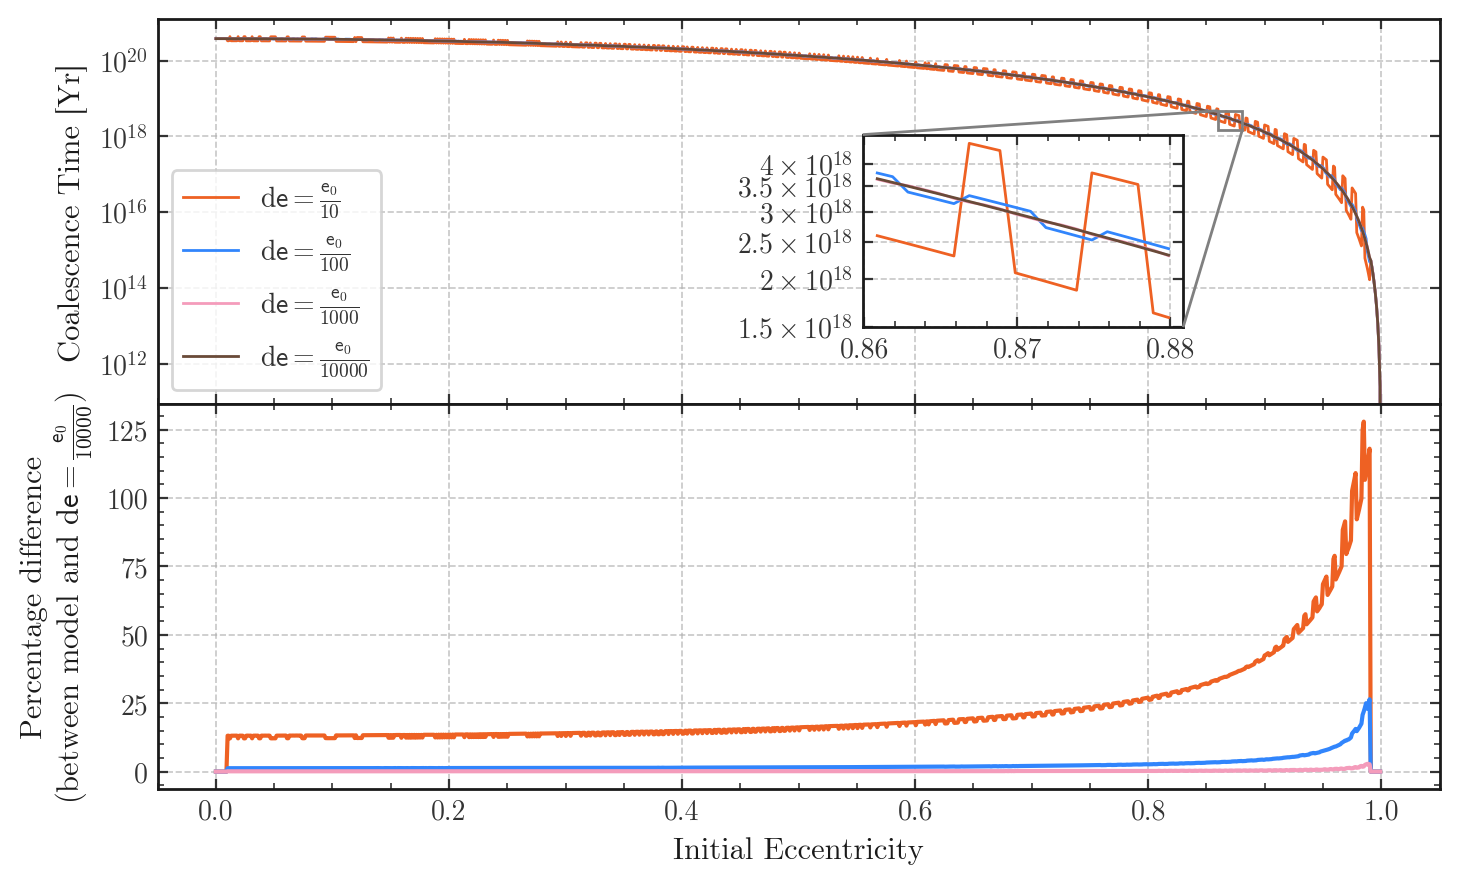
\includegraphics[width=\textwidth]{images/NatalKicks/varying_de.png}
    \caption[The effect of varying $\mathrm{d}e$ in \autoref{eq:discrete_sum} on the coalescence time.]{The effect of varying $\mathrm{d}e$ in \autoref{eq:discrete_sum} on the coalescence time. Although hard to see, the pink line does oscillate above and below the brown line. This binary was assumed to have $m_1=m_2=\SI{1.44}{\msun}$ and $a_0=\SI{1970.5}{\rsun}$ (the mean separation of a sample of binaries with $\alpha=\SI{100}{\km\per\s}, \beta=\SI{-170}{\km\per\s}$).}
    \label{fig:vary_de}
\end{figure}

\begin{figure}[!htbp]
    \centering
    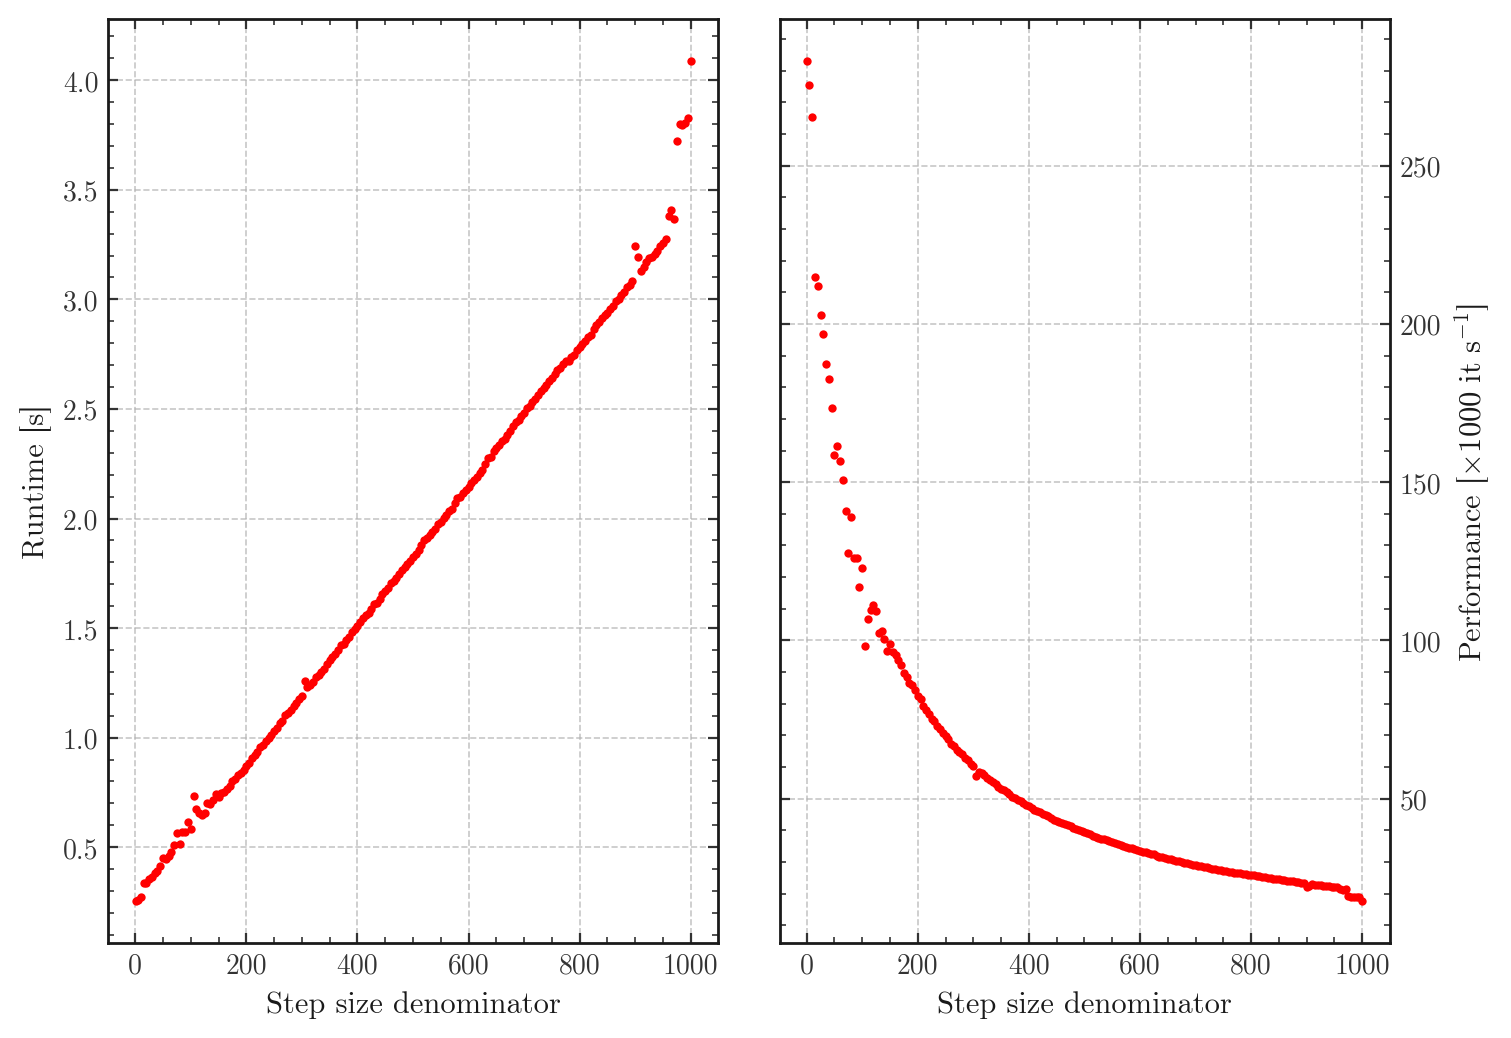
\includegraphics[width=\textwidth]{images/NatalKicks/runtime.png}
    \caption[The effect of varying $\mathrm{d}e$ in \autoref{eq:discrete_sum} on the runtime and performance.]{The effect of varying $\mathrm{d}e$ in \autoref{eq:discrete_sum} on the runtime, which is demonstrably $\mathcal{O}(n)$, and the performance of the algorithm. The input data to this algorithm were the LISA binary sample from Tang (priv. comm.). The performance is shown in units of thousands of iterations per second.}
    \label{fig:algo_runtime}
\end{figure}


\section{Merger Rates of BNS systems}\label{sec:merger_rates}

The first test is to match the observed merger rates of \gls{bns} systems. To do this, we use the \gls{lvk} catalogue of results from \gls{o3}. The simplest test is to match the merger rate today, which we denote as $\mathcal{R}_0$, to that observed by \gls{lvk} \citep{LIGOVirgo:2021a, LIGOVirgo:2021b}. We display this in \autoref{fig:merger_rates} alongside the previously reported fiducial values of $\alpha=\SI{100}{\km\per\s}$ and $\beta=\SI{-170}{\km\per\s}$, the theoretical merger rate calculation performed by \citet{Eldridge:2019}, and the observed merger rates from \citet{LIGOVirgo:2021a} and \citet{LIGOVirgo:2021b}. We term the contour defined by \citet{LIGOVirgo:2021a} (in black) the ``\gls{ligo} contour''.

Selecting the value to calibrate to is not a straightforward task. Although the \citet{LIGOVirgo:2021a} contour is superseded by the \citet{LIGOVirgo:2021b} contour, the separation into different inference models means that the merger rates for \gls{bns} systems have intractably large error bars covering the entire plane; for instance, their \textsc{MultiSource} (MS) model alone spans $2.11\leq\log\mathcal{R}_0\leq3.23$ which covers \textsc{FineGrid} entirely and almost entirely covers \textsc{WideGrid}. In addition to the lack of constraint, we would be imposing additional parameters into the model insofar as the selection of model -- whether, for example, PDB was taken as truth over BGP, MS, or one of the other population models. Whilst an interesting and assuredly insightful endeavour, the aim of this work is instead to develop a simple test that can be used in future on extra populations such as these. A simple criterion which can be extended is valuable, and future work may extend these tests in multiple directions.

\begin{figure}[!htbp]
    \centering
    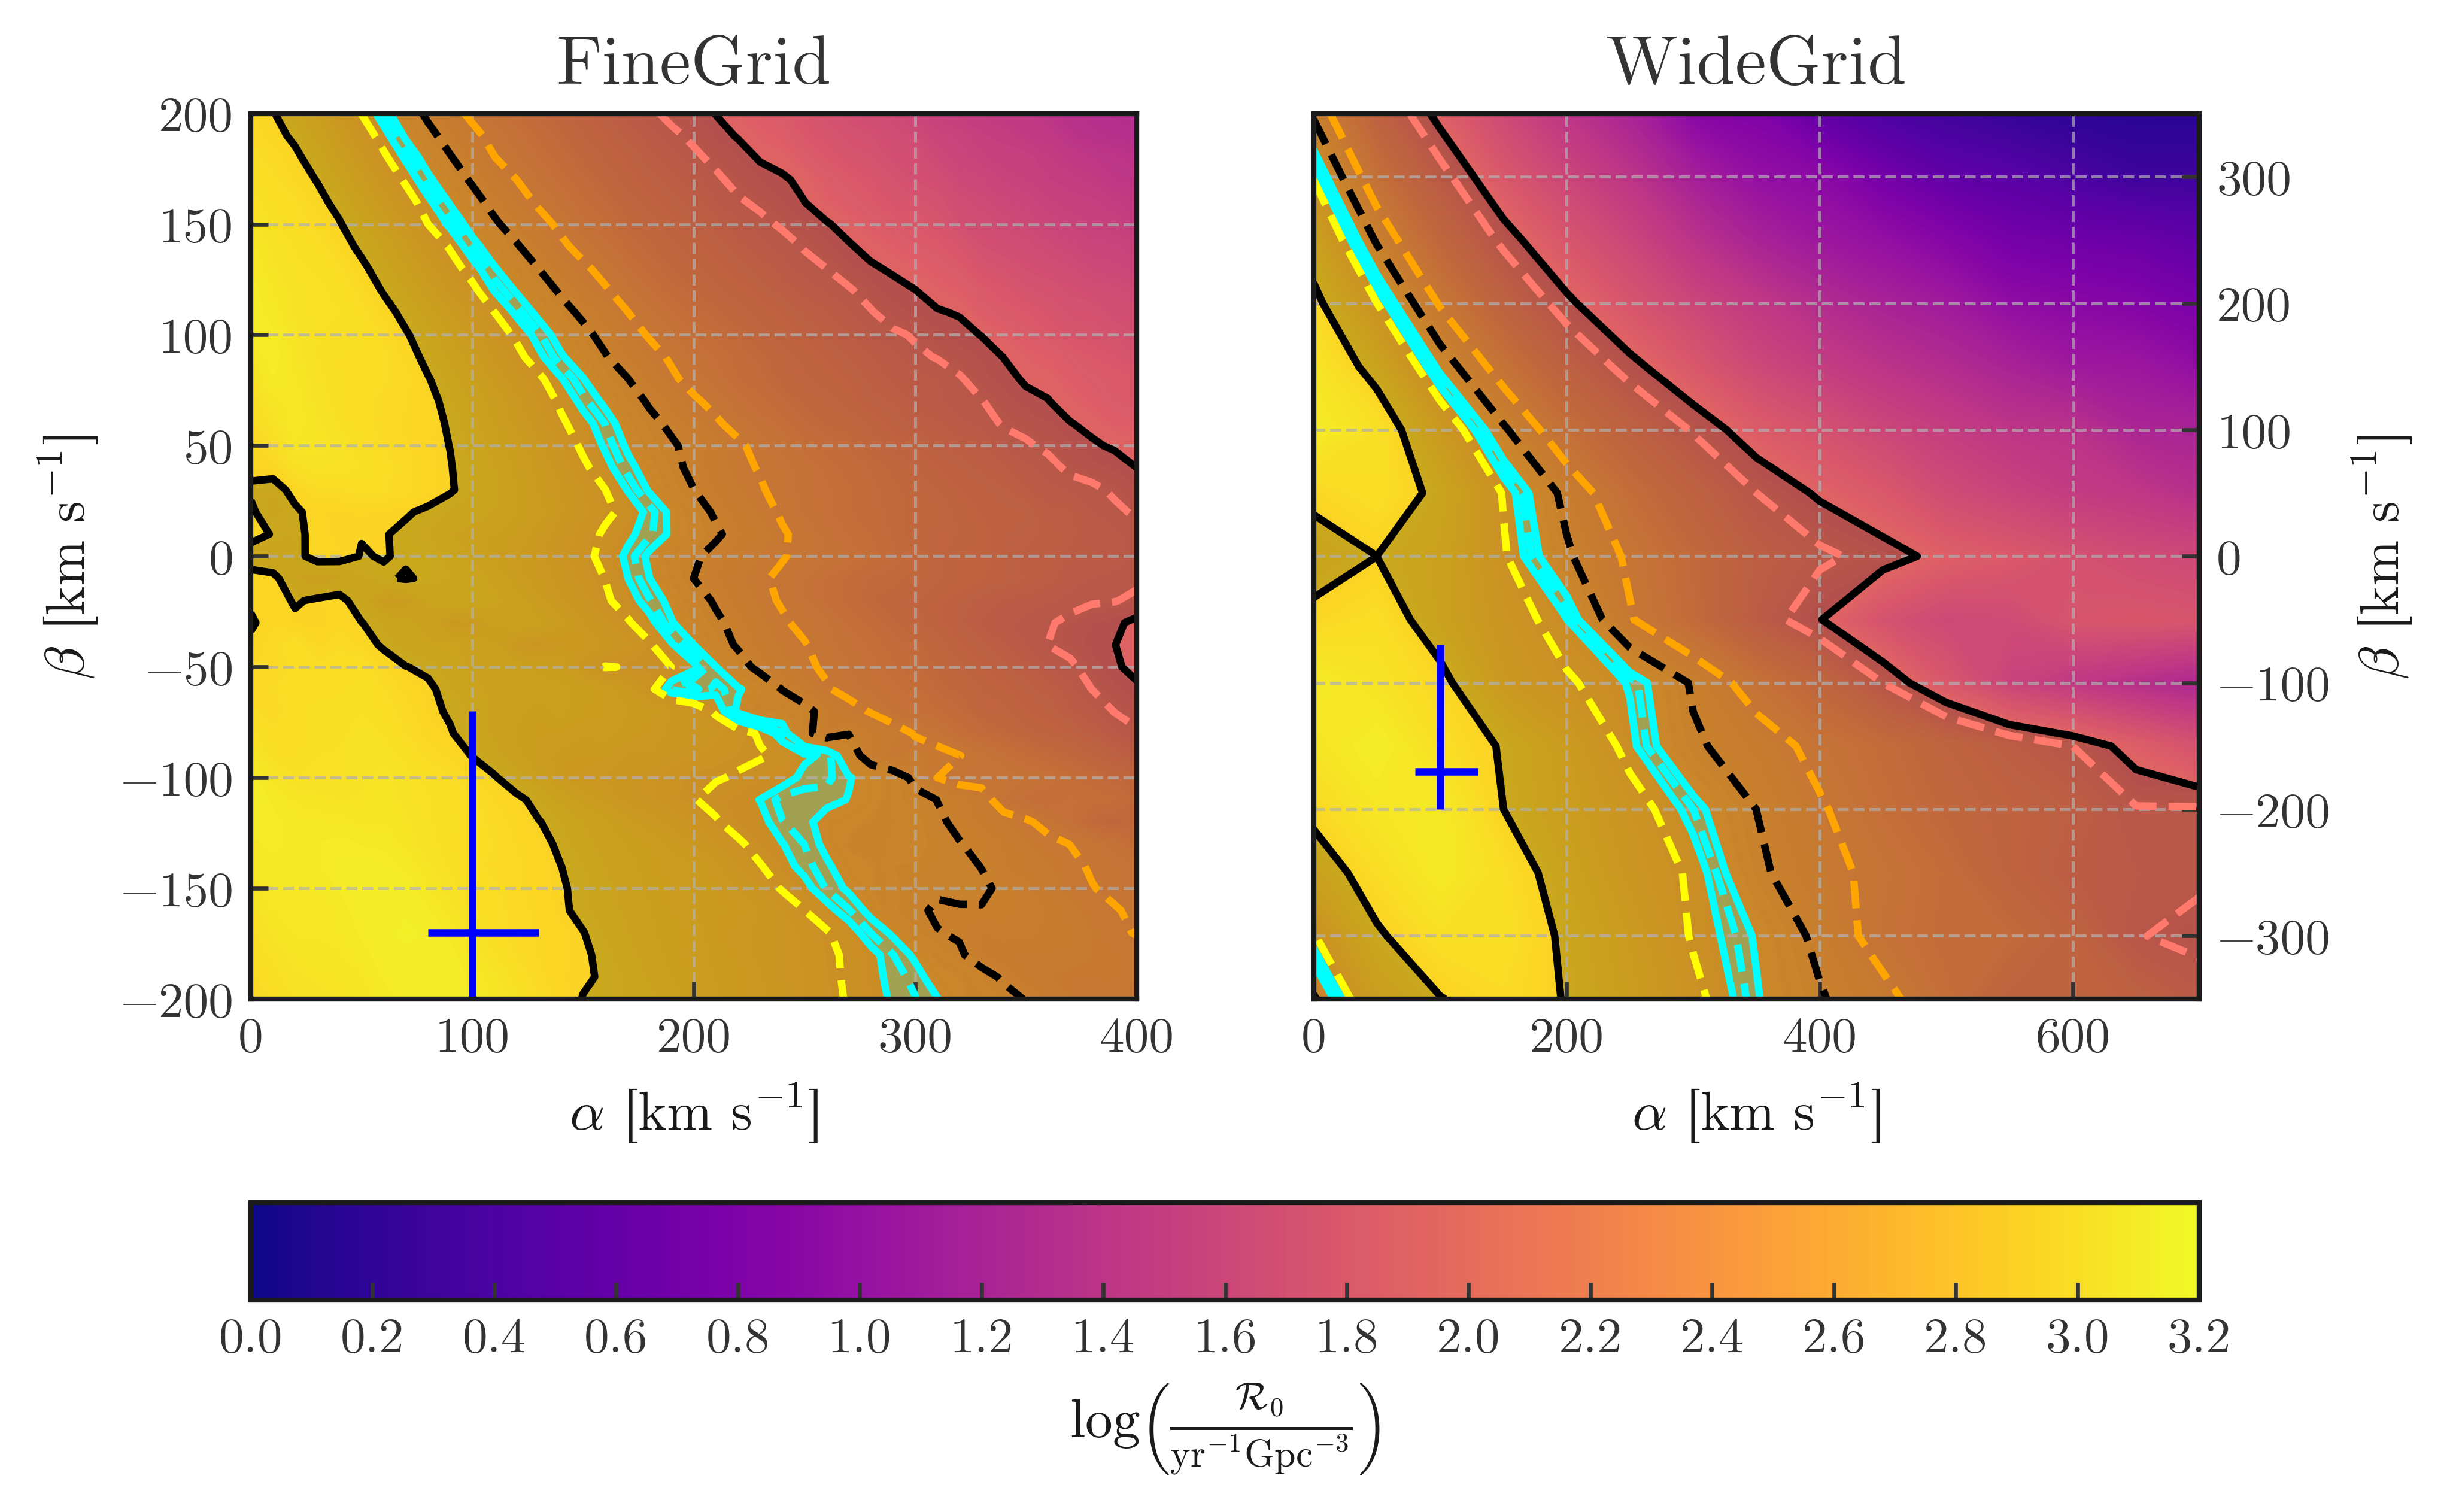
\includegraphics[width=\textwidth]{images/NatalKicks/EventRate_Distribution_Both.png}
    \caption[The merger rate as a function of kick parameters $\alpha$ and $\beta$.]{The merger rate as a function of kick parameters $\alpha$ and $\beta$. The cyan contour is the theoretical merger rate as reported by \citet{Eldridge:2019}. The black contour is the merger rate observed in \citet{LIGOVirgo:2021a}. The remaining contours are the merger rates reported in \citet{LIGOVirgo:2021b} (pink: BGP, yellow: MS, orange: PDB [ind], see \citet{LIGOVirgo:2021b} for an explanation of each model). Shaded regions represent uncertainties, and uncertainties are not reported for the \citet{LIGOVirgo:2021b} results as they would cover the entire plane. The blue cross is the fiducial value of $\alpha$ and $\beta$ from \citet{Bray:2018}. This value lies off the previous work's contours as the rejuvenation age calculation has been improved in \codename{Tui} in preparation for the next major BPASS release.}
    \label{fig:merger_rates}
\end{figure}

\section{Period-Eccentricity Distributions}\label{sec:per_ecc_dist}

Since in the absence of any mass transfer the motion of two compact binaries is wholly dependent on their initial separation and orbital eccentricity, they trace out paths in a two-dimensional phase space. In general, since binaries circularise over time, and by the emission of gravitational waves their orbits shrink, a binary will start in the high-period, high-eccentricity region of period-eccentricity space, and evolve towards the low-period, low-eccentricity region. As a result, given a population of binary stars, we can design a density plot, where the density is effectively the likelihood of a binary selected at random having the parameters we sample.

\begin{figure}[!htbp]
    \centering
    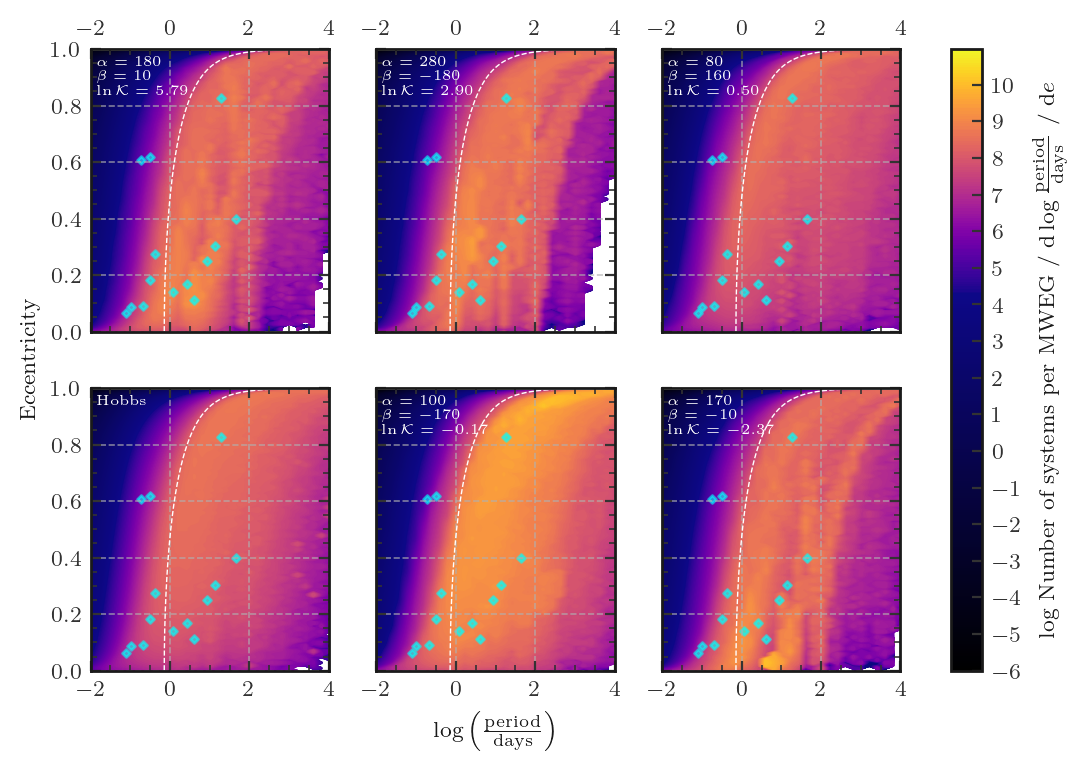
\includegraphics[width=\textwidth]{images/NatalKicks/PE_dists_six_panel.png}
    \caption[The period-eccentricity distributions for six selected \citet{Bray:2016} kicks.]{The period-eccentricity distributions for six selected \citet{Bray:2016} kicks. Shown are the kicks for $\alpha=\SI{180}{\km\per\s}, \beta=\SI{10}{\km\per\s}$ as the system with the highest $\ln\mathcal{K}$ across the \gls{ligo} contour, $\alpha=\SI{170}{\km\per\s}, \beta=\SI{-10}{\km\per\s}$ as the lowest, and the balance to illustrate structural differences. White regions show regions where no systems evolve to. The white line represents a constant-time coalescence time of the Hubble time ($\sim\SI{13.8}{\giga\year}$), computed using \citet{Mandel:2021a}. The cyan diamonds are the observed systems enumerated in \autoref{tab:observed_BNSes}. In white text are the values of $(\alpha,\beta)$, and the $\ln\mathcal{K}$ values for each plot.}
    \label{fig:6panel-pe_dists}
\end{figure}

Computationally, for each binary in our sample, we trace its path through period-eccentricity space, and at every timestep we add $w\times{\rm d}t$ to the density plot, where ${\rm d}t$ is the timestep, and $w$ is the weight term output from the \codename{Tui} code proportional to the \gls{imf} weight (where the constant of proportionality is related to the uniformly sampled kick direction). The result of this computation, for the parameter values that lie along the \gls{ligo} contour, are shown in \autoref{chap:ligo_contour_results}. We also show the same result in \autoref{fig:6panel-pe_dists}.  Given a catalogue of $N$ (observed) binary stars, we can then compute the likelihood of the model as

\begin{equation}
    \ln \mathcal{L} = \sum_{n=0}^N \ln p\left(\ln P_n, e_n\right),\label{eq:log_likelihood_summand}
\end{equation}

where $p\left(\ln P_n, e_n\right)$ is the content of the density plot at the location of the $n^\text{th}$ observed \gls{bns} system. Then, the Bayes factor (defined as the likelihood ratio) can be computed as

\begin{equation}
    \mathcal{K}\equiv\frac{\mathcal{L}}{\mathcal{L}_\text{Hobbs}} \implies \ln\mathcal{K} = \ln\mathcal{L}-\ln\mathcal{L}_\text{Hobbs},
\end{equation}

where $\mathcal{L}_\text{Hobbs}$ is the log-Likelihood of the Hobbs kick. We use a catalogue of fourteen \gls{bns} systems originally compiled in \citet{Vigna-gomez:2018}, shown in \autoref{tab:observed_BNSes}. From this catalogue, we sample the period-eccentricity distribution at that space and take that as the probability of observing that binary, thus allowing us to use the content of the period-eccentricity distribution as the $\ln p$ term in our summand of \autoref{eq:log_likelihood_summand}.

By doing this we effectively construct a Bayes-factor map, where $\ln\mathcal{K}$ can be shown evaluated at every combination of $\alpha$ and $\beta$. We term this value $\ln\mathcal{K}_{\alpha\beta}$. This is shown in \autoref{fig:log_bayes_both} for both of our considered grids. In general we see that approximately 60\% of \textsc{FineGrid} has a positive log-Bayes factor (indicating any level of support of the model compared to Hobbs), whereas approximately 40\% of \textsc{WideGrid} has a positive log-Bayes factor. In a Bayesian analysis, the constraint that $\ln\mathcal{K} \geq 3.4$ indicates strong support for the model contrasted against the reference \citep[i.e.,][]{Hobbs:2005}, which contains approximately 9.1\% of \textsc{FineGrid} and 4.4\% of \textsc{WideGrid}.

\begin{table}
    \centering
    \small
    \tabcolsep=0.11cm
    \begin{tabular}{cccc||cccc}
        \hline
        Name & $\log (P / \text{days})$ & $e$ & Original Reference & Name & $\log (P / \text{days})$ & $e$ & Original Reference \\
        \hline
         J0453+1559 &  0.609808 &  0.113 & \citet{Martinez:2015}       & J0737-3039 & -0.991400 &  0.088 & \citet{Kramer:2006} \\
           B1534+12 & -0.375718 &  0.274 & \citet{Fonseca:2014} & J1756-2251 & -0.494850 &  0.181 & \citet{Faulkner:2005} \\
           B1913+16 & -0.490797 &  0.617 & \citet{Hulse:1975}       & J1913+1102 & -0.686133 &  0.090 & \citet{Lazarus:2016} \\
         J1757-1854 & -0.735182 &  0.606 & \citet{Cameron:2018}          & J1518+4904 &  0.936212 &  0.249 & \citet{Janssen:2008} \\
         J1811-1736 &  1.273672 &  0.828 & \citet{Corongiu:2007}       & J1829+2456 &  0.070407 &  0.139 & \citet{Champion:2004} \\
         J1930-1852 &  1.653791 &  0.399 & \citet{Swiggum:2015}           & J1753-2240 &  1.134751 &  0.304 & \citet{Keith:2009} \\
         J1411+2551 &  0.417638 &  0.169 & \citet{Martinez:2017}       & J1946+2052 & -1.107905 &  0.064 & \citet{Stovall:2018} \\
        \hline
    \end{tabular}
    \caption[The systems we use in our study.]{The systems we use in our study. These data were originally compiled in \citet{Vigna-gomez:2018}.}
    \label{tab:observed_BNSes}
\end{table}

\begin{figure}[!htbp]
    \centering
    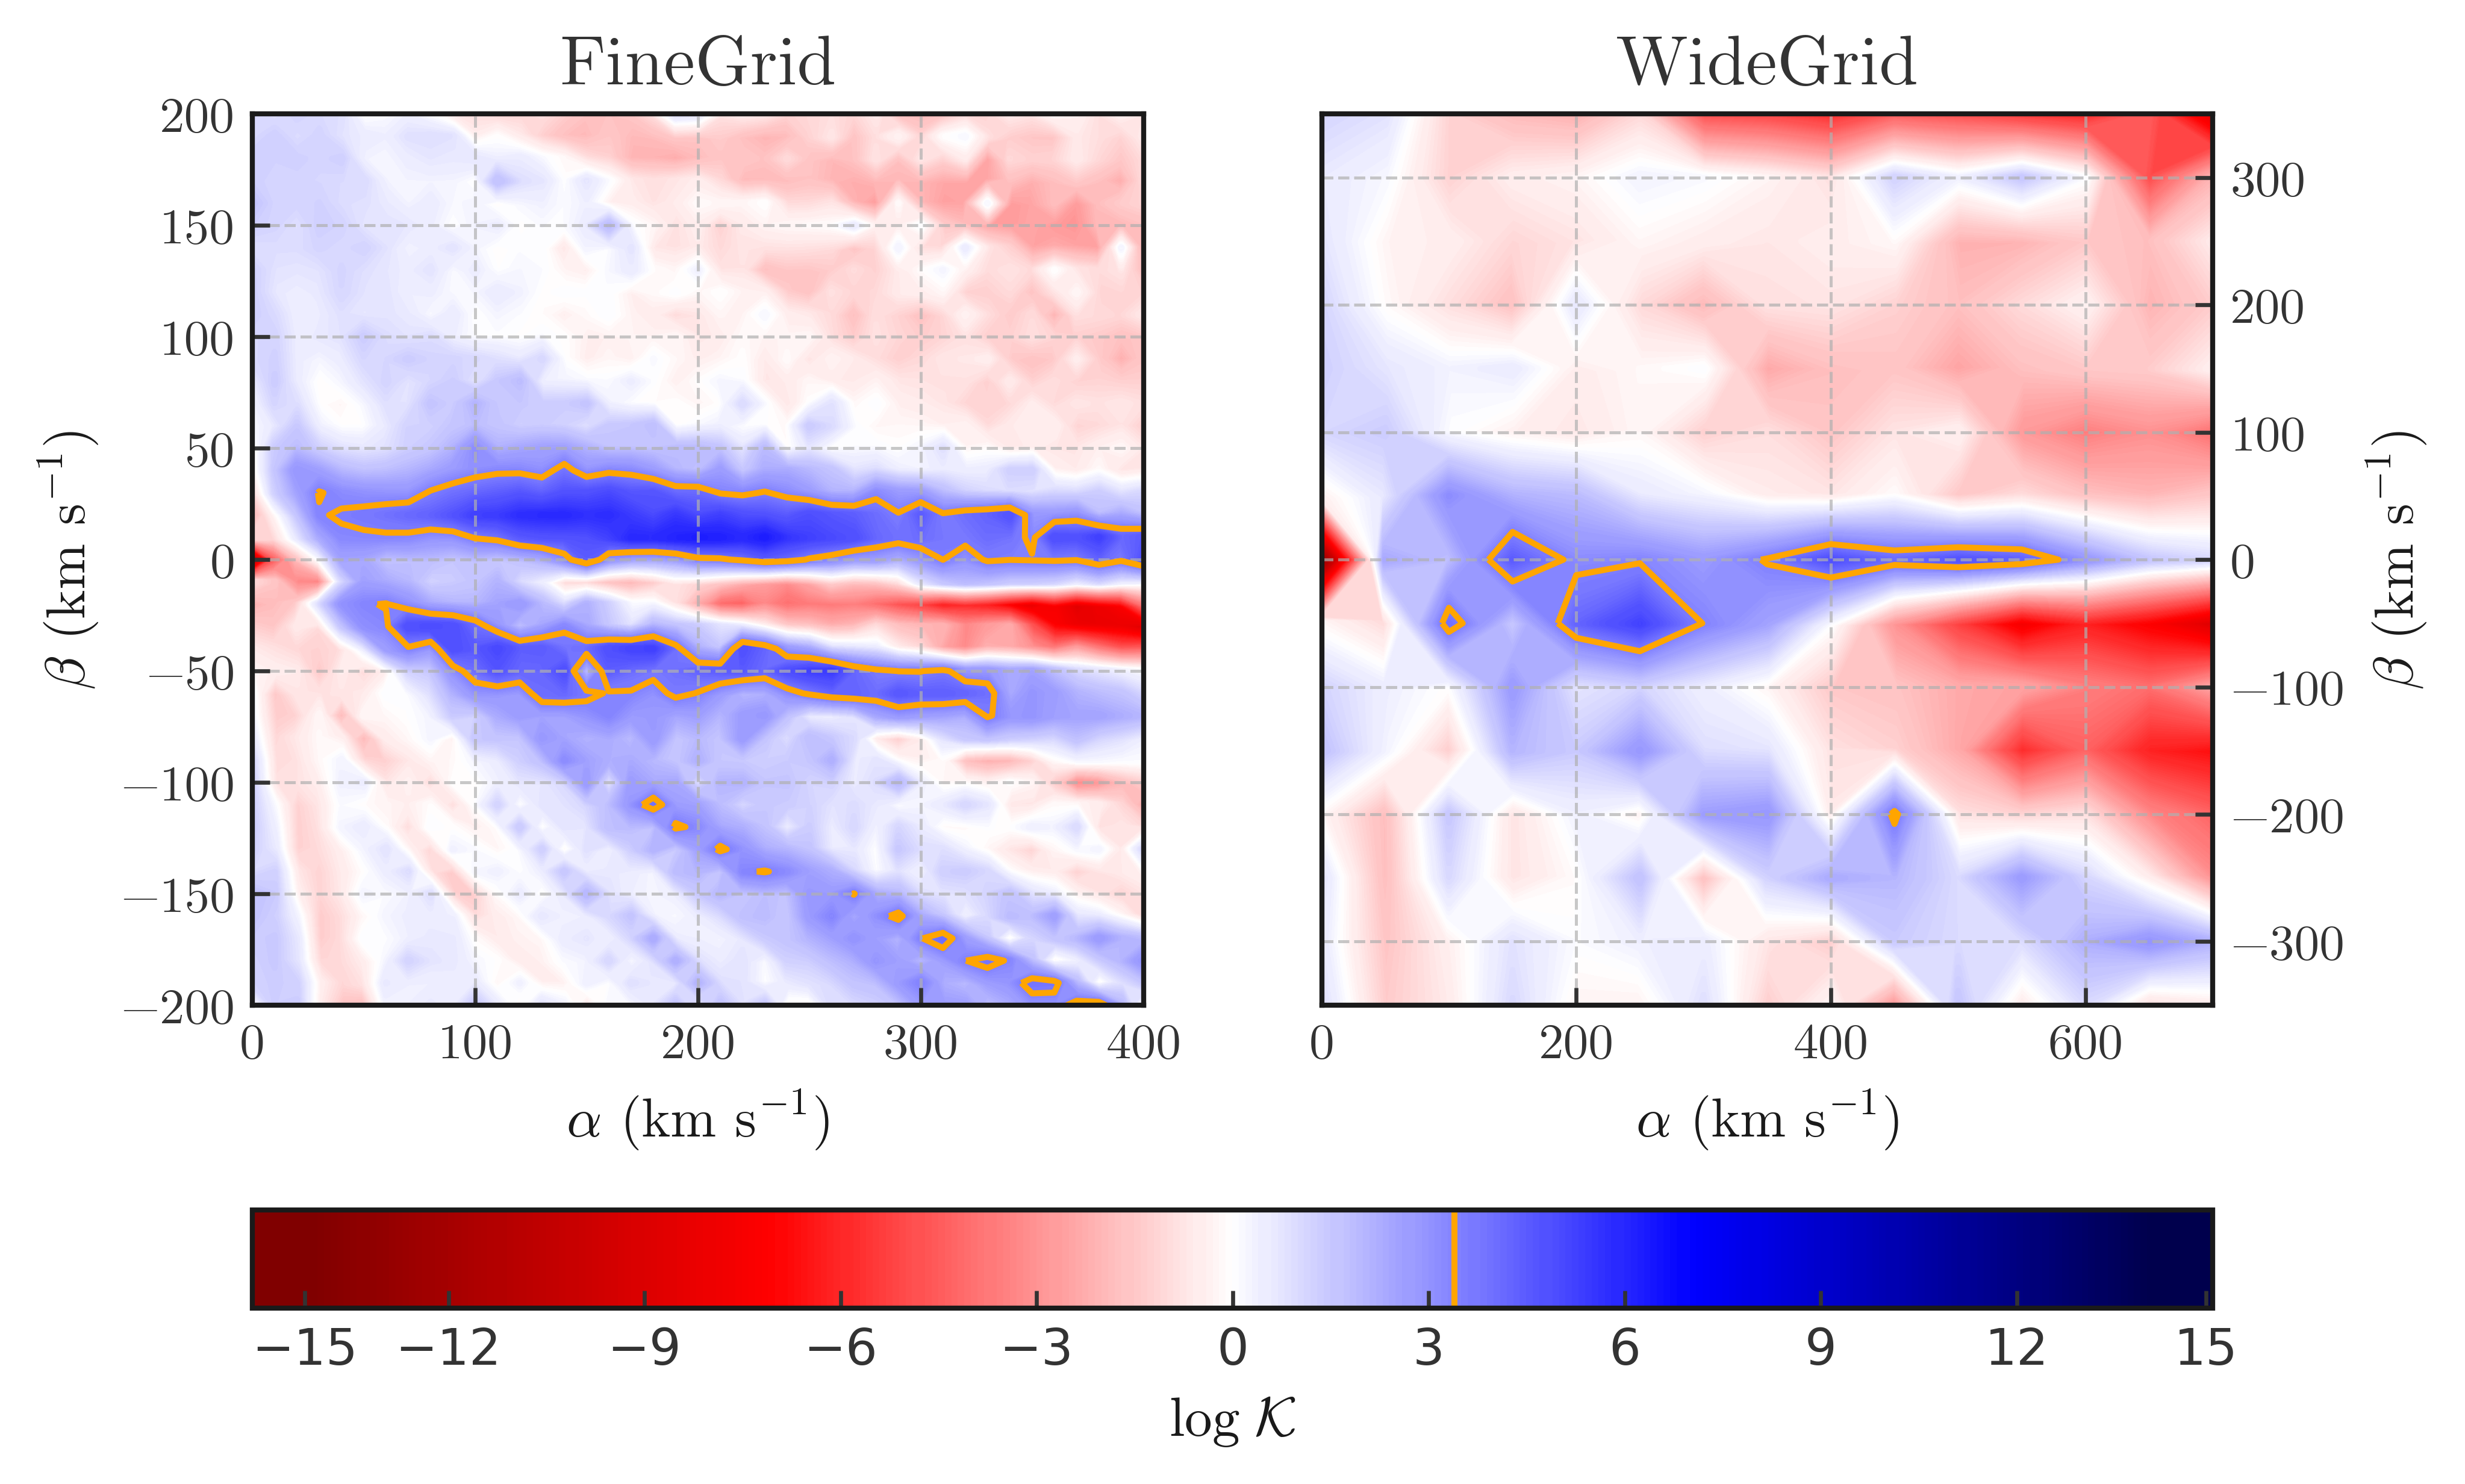
\includegraphics[width=\textwidth]{images/NatalKicks/LogBayesFactors_Both.png}
    \caption[The $\ln\mathcal{K}$ values across $\alpha-\beta$ space.]{The $\ln\mathcal{K}$ values across $\alpha-\beta$ space. The orange line demarcates $\ln\mathcal{K}=3.4$, which in a Bayesian test represents conclusive evidence in favour of the distribution compared to the \citet{Hobbs:2005} kick.}
    \label{fig:log_bayes_both}
\end{figure}

\section{Single-Star Kick Velocities}\label{sec:ssk_vels}

The traditional methodology for refining a kick prescription is to consider the velocity distribution of isolated pulsars. Thus, given a suitable observational dataset, we would be able to compute the expected kick distribution and compare it, via a \gls{ks} test, to the observed data set. The \gls{ks} statistic between distributions $\mathcal{F}$ (the observed distribution) and $\mathcal{G}$ (the compared distribution) is given by

\begin{equation}
        \text{KS} = \max\left|\text{cdf}(\mathcal{F})-\text{cdf}(\mathcal{G})\right|,
\end{equation}

where cdf means the \gls{cdf} function, defined as the integral of the \gls{pdf}. Given the \gls{cdf} is bounded between 0 and 1 inclusive, the \gls{ks} statistic is also bounded between this region. A \gls{ks} statistic of 1 means that the compared distribution diverges perfectly from the observed distribution, whereas a \gls{ks} statistic of 0 means it matches perfectly. This test of divergence was the refinement performed in \citet{Bray:2016, Bray:2018}, hence we select this (with an independently generated dataset to those works) to be consistent with prior work.

\subsection{Pulsar velocity dataset}

We use the same dataset of 81 pulsars from \citet{Willcox:2021}, and filter the dataset in the same way that they do. We remove millisecond pulsars, pulsars in globular clusters, and pulsars known to be in binaries, in order to homogenise the dataset. The \gls{pdf} and \gls{cdf} of \citet{Willcox:2021}, as well as those generated from \citet{Hobbs:2005} and \citet{Bray:2018}, is displayed in \autoref{fig:bray_vs_hobbs_vs_willcox_pdf}.

This homogenised dataset gives the transverse velocities of each pulsar alongside the RA/Dec, the proper motion in the RA/Dec directions, and parallax. We assume that the transverse velocity is approximately the original kick velocity. As mentioned earlier in this chapter, old remnants with high velocities may have moved substantially -- a \SI{20}{\mega\year} remnant with a transverse velocity of $\SI{500}{\km\per\s}$ will have moved $\sim\SI{10}{\kilo\pc}$, absent external forces \citep{Willcox:2021}. However, this is likely only to be an issue for pulsars whose transverse velocity substantially exceeds the transverse Galactic rotational velocity of the Sun $v_\text{TGRV}\approx\SI{230}{\km\per\s}$ \citep{Bhattacharjee:2014}, shown in yellow on \autoref{fig:bray_vs_hobbs_vs_willcox_pdf}. Although the dataset of \citet{Willcox:2021} has pulsars with velocities higher than this value -- peaking at $\sim\SI{850}{\km\per\s}$ -- this is not a grave concern for this work, for two reasons. Firstly, the kick velocities output from \codename{Tui} are taken immediately after the supernova. Secondly, the analysis \citet{Willcox:2021} performs is focused on low-velocity pulsars, and this test limits the kick velocity of an \glspl{ussne} to \SI{30}{\km\per\s}, well below $v_\text{TGRV}$.

\begin{figure}[!htbp]
    \centering
    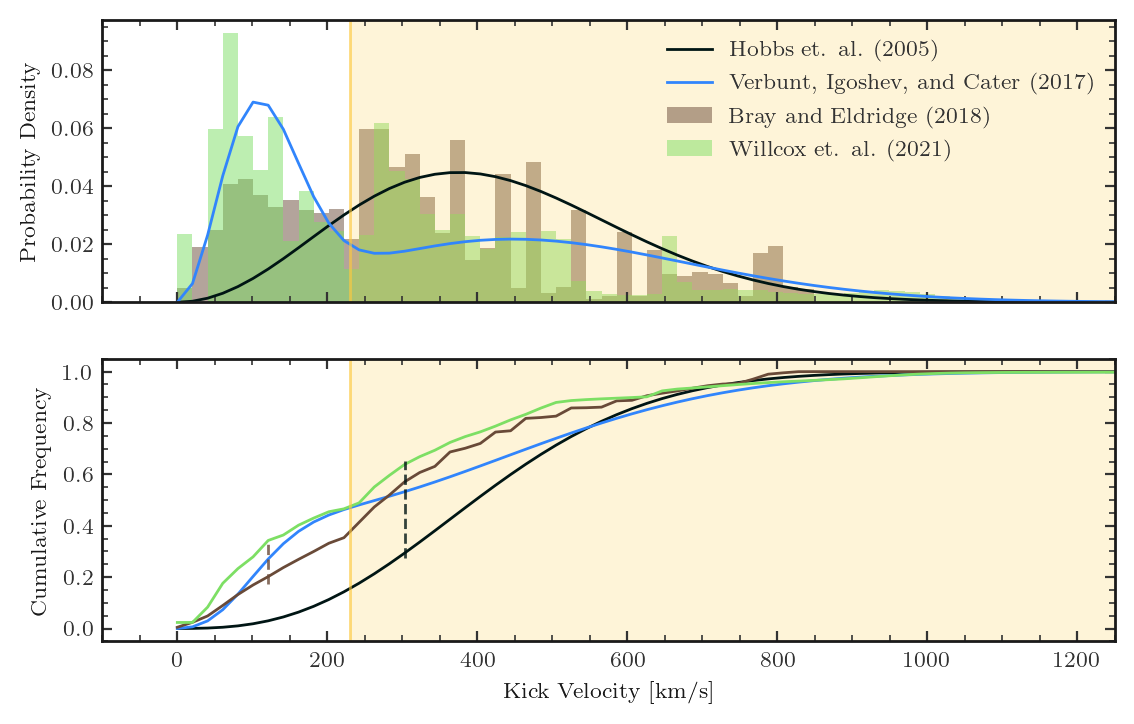
\includegraphics[width=\textwidth]{images/NatalKicks/bray_vs_hobbs.png}
    \caption[The \acrshort{pdf} and \acrshort{cdf} of the distributions using kicks from \citet{Hobbs:2005, Verbunt:2017, Bray:2018, Willcox:2021}.]{The \gls{pdf} and \gls{cdf} of the distributions using kicks from \citet{Hobbs:2005, Verbunt:2017, Bray:2018, Willcox:2021}. \citet{Hobbs:2005} has a closed-form expression, whereas the others are computed empirically, hence the Bray and Willcox \acrshortpl{cdf} are less smooth than that of Hobbs. The two dashed lines indicate where and how the \gls{ks} statistic is measured for the associated distribution. The yellow region indicates the region for which $v_\text{kick}\geq v_\text{TGRV}$, the transverse Galactic rotation velocity of the Sun, $\sim\SI{230}{\km\per\s}$.}
    \label{fig:bray_vs_hobbs_vs_willcox_pdf}
\end{figure}

The \citet{Hobbs:2005} kick has a closed-form expression for the \gls{pdf} $P(v_\text{k})$, given by \autoref{eq:hobbs_kick}. Consequently, it has a smooth curve in \autoref{fig:bray_vs_hobbs_vs_willcox_pdf}, whereas the \citet{Bray:2018} and \citet{Willcox:2021} \glspl{pdf} are presented as histograms as they are computed.

\begin{figure}[!htbp]
    \centering
    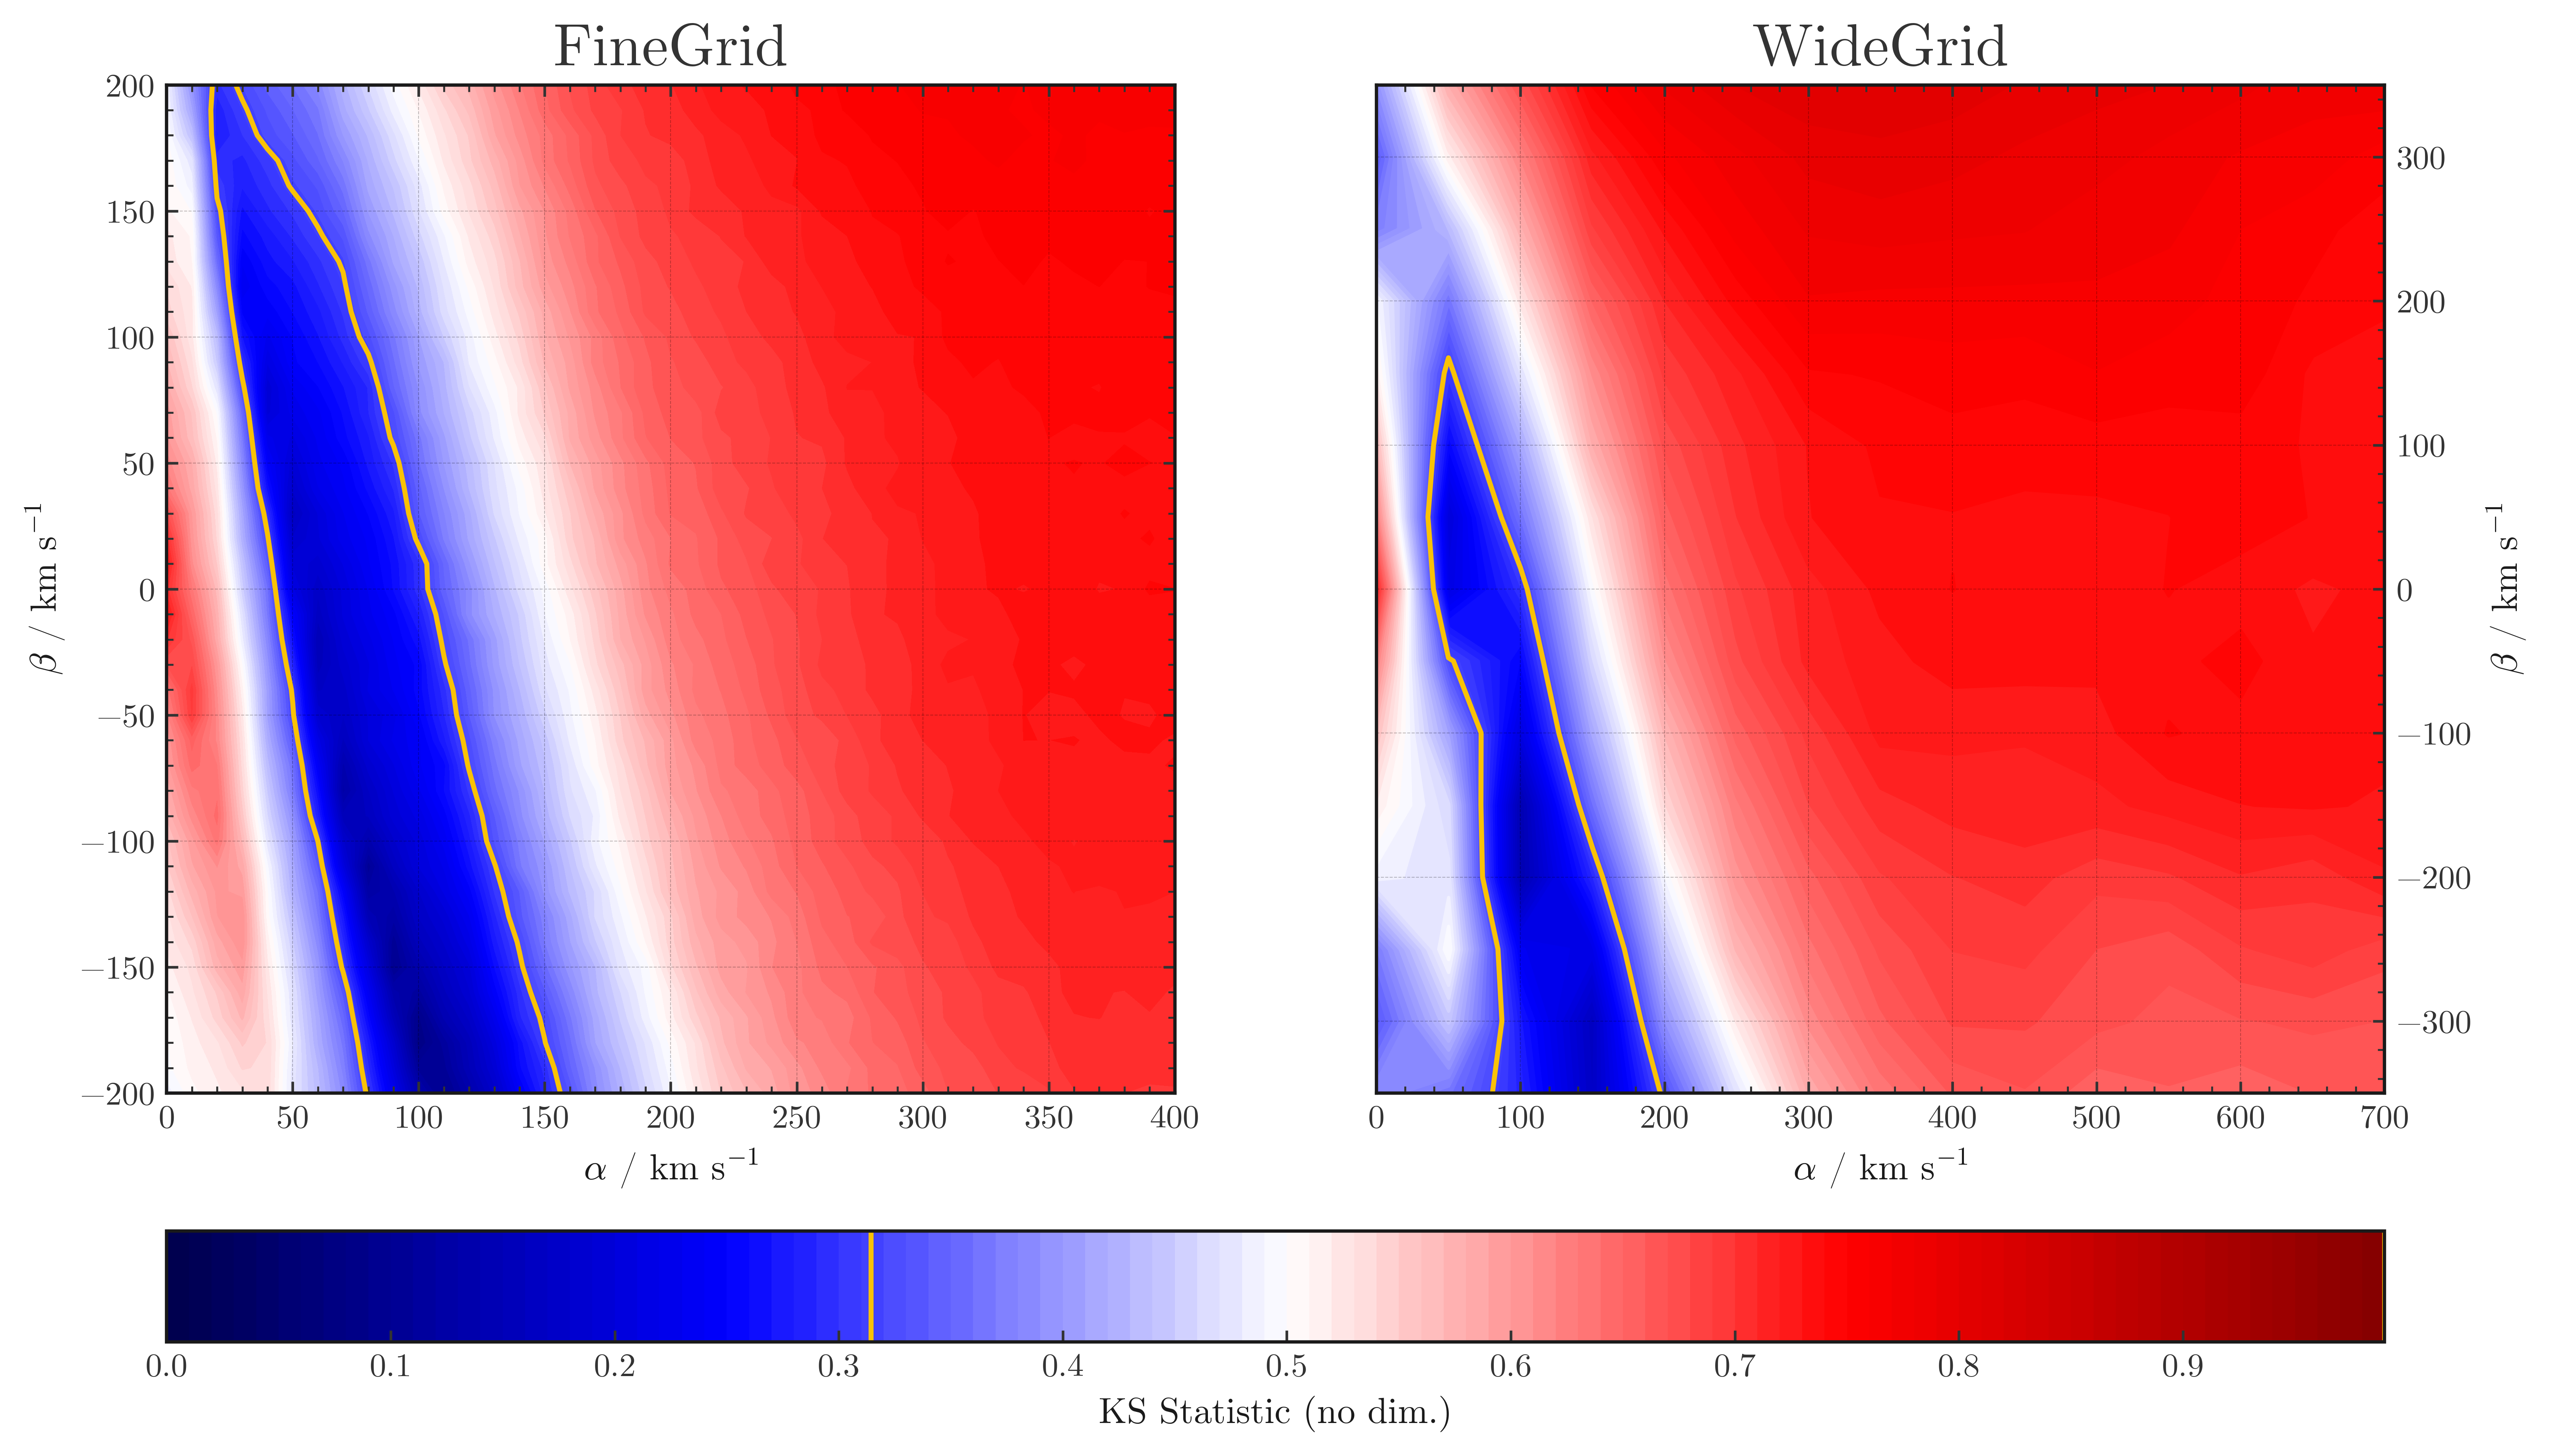
\includegraphics[width=\textwidth]{images/NatalKicks/ks_test.png}
    \caption[The \acrshort{ks} statistic for \textsc{FineGrid} and \textsc{WideGrid}.]{The \gls{ks} statistic for \textsc{FineGrid} and \textsc{WideGrid}. The orange line denotes the \gls{ks} statistic for the Hobbs kick, which has a value of 0.34.}
    \label{fig:ks_test_with_hobbs}
\end{figure}

\subsection{Comparison}

\autoref{fig:ks_test_with_hobbs} shows the \gls{ks} statistic as a function of $\alpha$ and $\beta$ across our two parameter spaces. We also show the \gls{ks} statistic of the Hobbs kick, which has a value of 0.34. We find in general a valley of models with good agreement to \citet{Willcox:2021}, and find that the global minimum \gls{ks} statistic is at $\alpha=100, \beta=-180$ -- agreeing with the prior work of \citet{Bray:2018} (who find $\alpha=100, \beta=-170$).

\begin{figure}[!htbp]
    \centering
    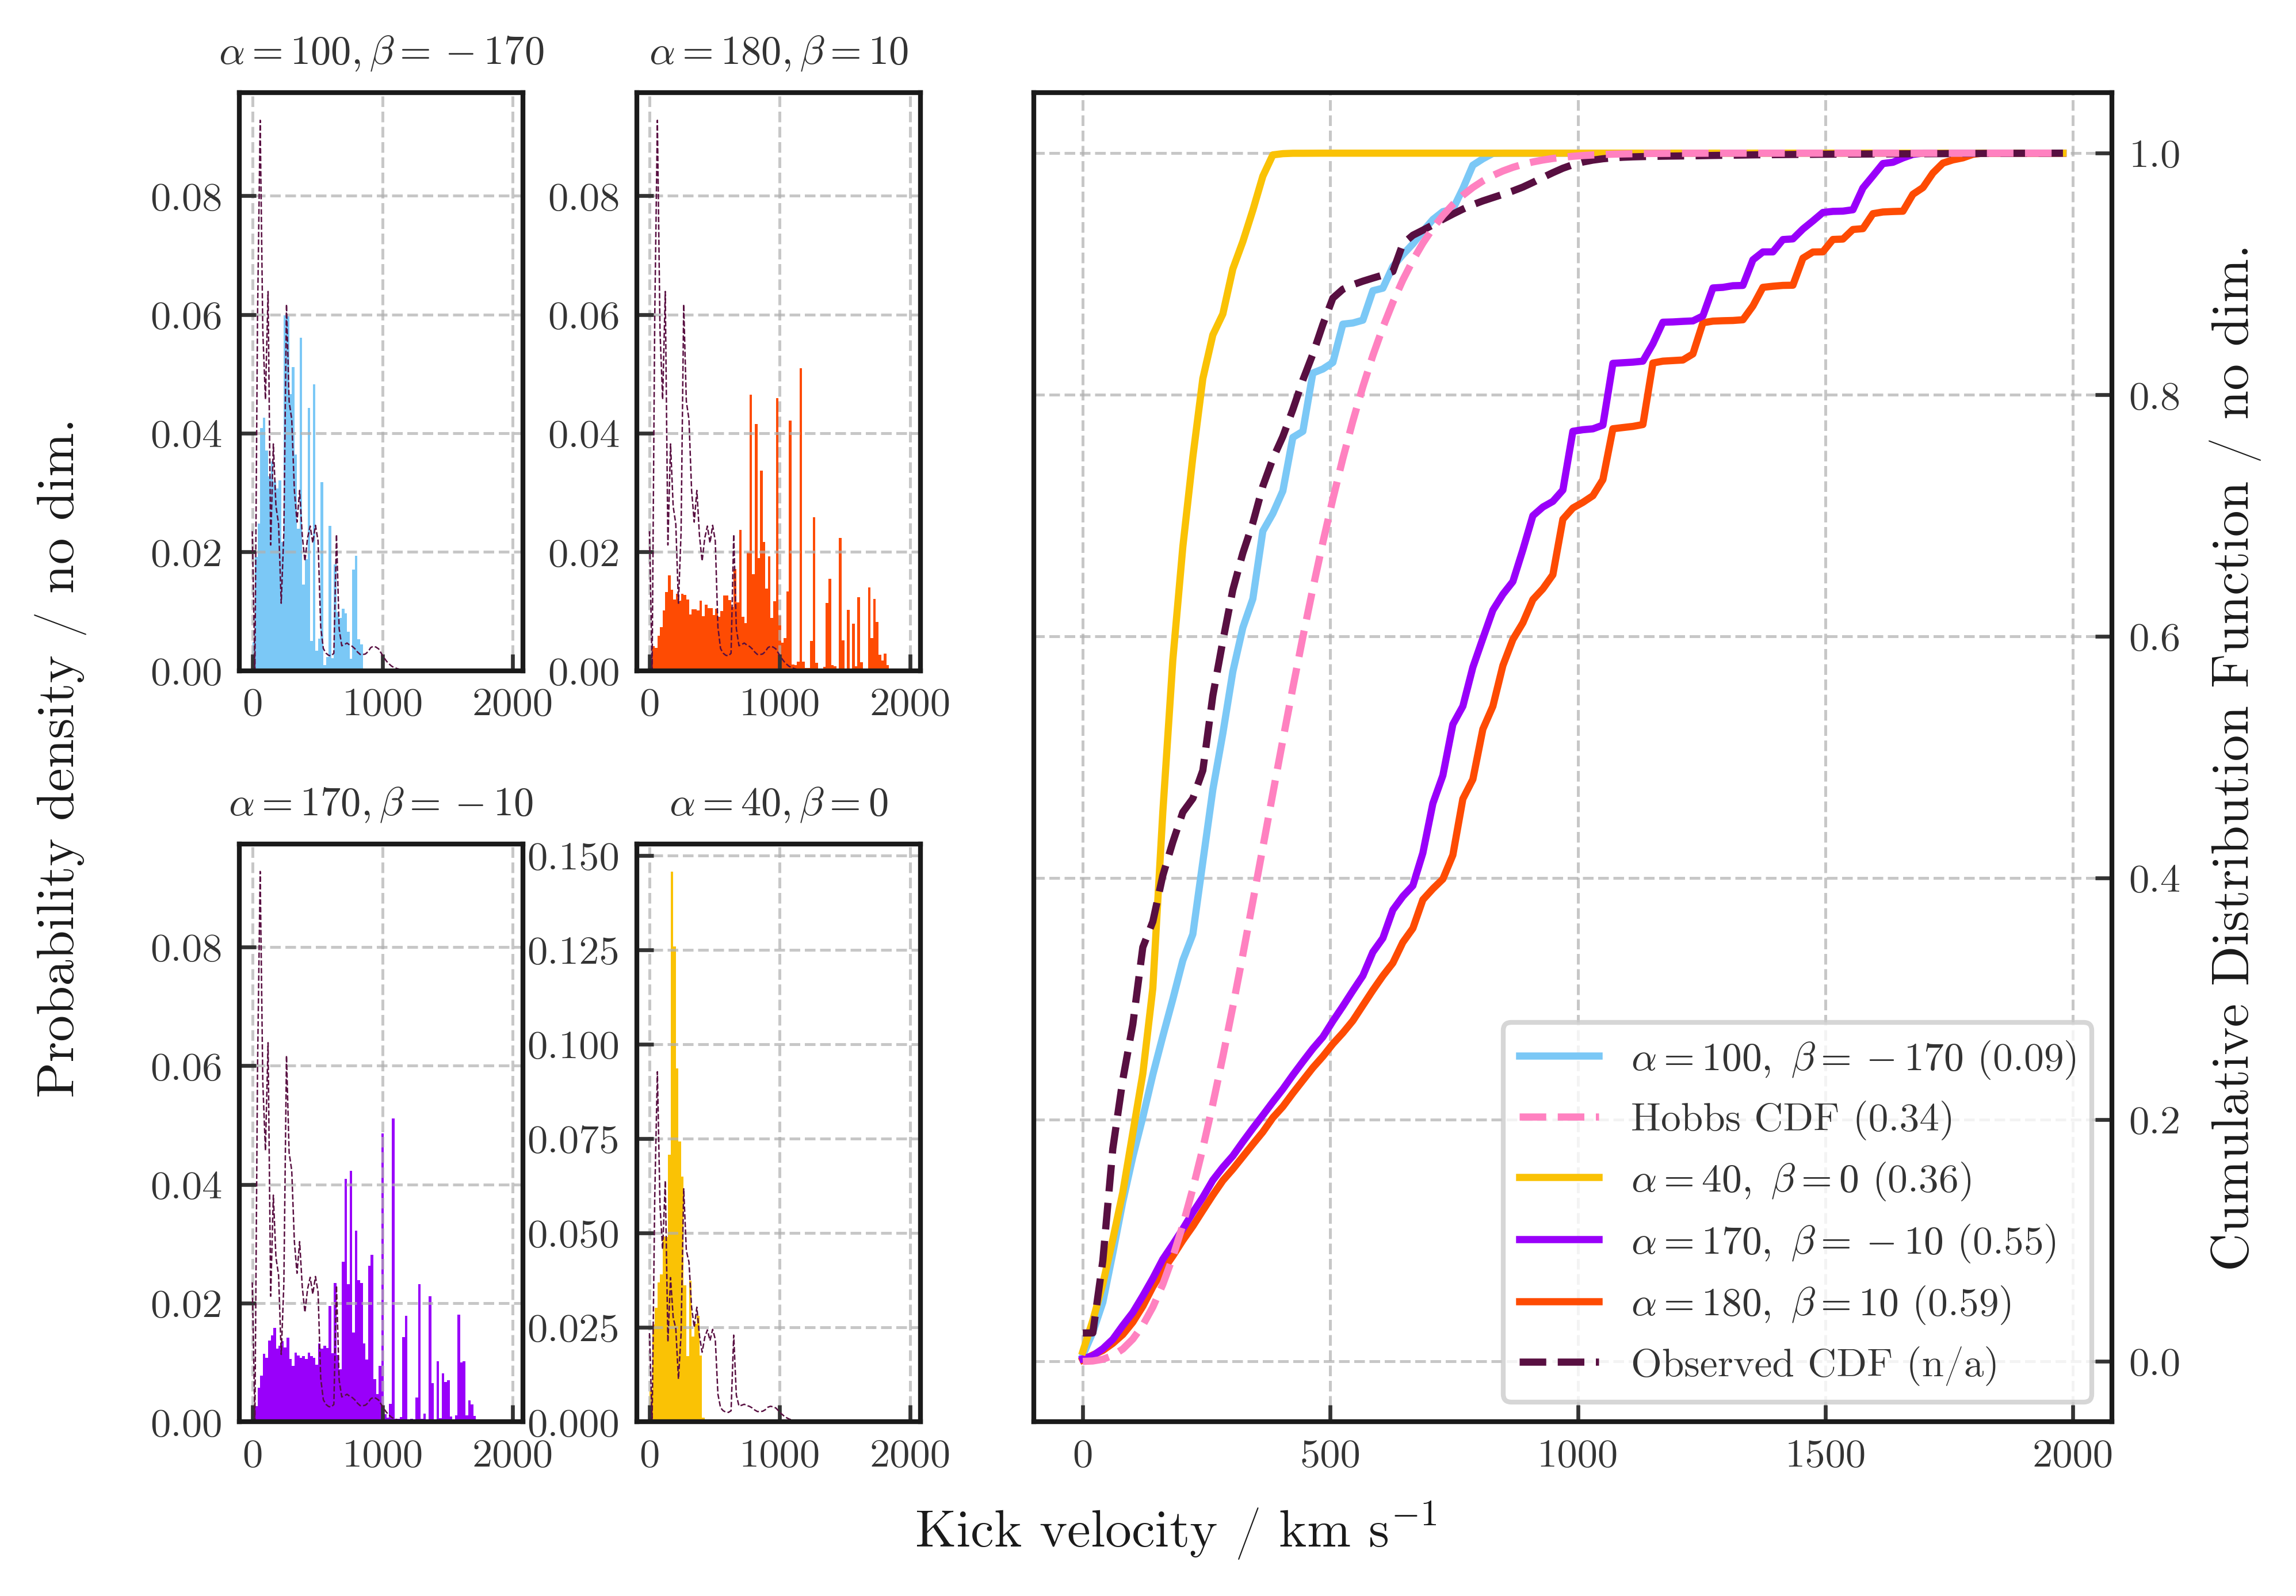
\includegraphics[width=\textwidth]{images/NatalKicks/individual_pdfs_with_cdf_and_hobbs.png}
    \caption[The \acrshortpl{pdf} and \acrshortpl{cdf} of four systems, alongside the Hobbs \acrshort{cdf} and \citet{Willcox:2021} \acrshort{cdf}.]{The \glspl{pdf} and \glspl{cdf} of four systems, alongside the Hobbs \gls{cdf} and \citet{Willcox:2021} \gls{cdf}. The dashed line on the \gls{pdf} plots is the \gls{pdf} of the observed distribution from \citet{Willcox:2021}. On the right hand plot, the number in parentheses represents the \gls{ks} statistic for the distribution, measured relative to \citet{Willcox:2021}, which by definition has no \gls{ks} statistic.}
    \label{fig:some_individual_pdfs}
\end{figure}

We also show in \autoref{fig:some_individual_pdfs} a selection of four \glspl{pdf}, alongside their associated \gls{cdf} and the \glspl{cdf} for \citet{Willcox:2021} and the Hobbs kick. We note that the numerical values shown in \autoref{fig:some_individual_pdfs} differs somewhat from those shown in \citet{Richards:2023}. This was due to a minor bug in the code incorrectly labelling the KS statistics for the figure. The actual result of the paper does not change with the correction of the bug, however the values reported in Figure 5 of \citet{Richards:2023} do change.

The four values we present on the left side of \autoref{fig:some_individual_pdfs} correspond to $\alpha = \SI{100}{\km\per\s}, \beta=\SI{-170}{\km\per\s}$ for the fiducial Bray kick, $\alpha = \SI{180}{\km\per\s}, \beta = \SI{10}{\km\per\s}$ to represent the system with the highest $\ln\mathcal{K}$ value from \autoref{sec:per_ecc_dist}, $\alpha = \SI{170}{\km\per\s}, \beta = \SI{-10}{\km\per\s}$ the lowest, and $\alpha = \SI{40}{\km\per\s}, \beta = \SI{0}{\km\per\s}$ the system with low $\alpha$ and zero $\beta$, corresponding to a kick that would \textit{a priori} generate logical velocities in the \glspl{ussne} limit.

\section{Production of Ultra-Stripped Supernovae}\label{sec:ussne_production}

As discussed earlier, the fiducial values of the Bray kick from \citet{Bray:2018} admit some problematic extremal cases. If $m_\text{ej}\to 0$, as is the case in a \gls{ussne}, the kick velocity would become negative. For instance, an ``average'' \gls{ussne} with $m_\text{ej}=\SI{0.15}{\msun}$ and $m_\text{rem}=\SI{1.45}{\msun}$ would have a kick velocity of $\sim\SI{-159}{\km\per\s}$. The concern here is twofold. Firstly, a negative kick velocity would mean that the velocity vector of the kick would be antialigned with the direction of the more massive remnant; this is a violation of conservation of momentum. Secondly, a kick with high magnitude means that, irrespective of the alignment of the kick, the kick itself is strong. As discussed in \citet{Willcox:2021}, \glspl{ussne} are associated with weak kicks, peaking at $v_\text{k}\sim\SI{30}{\km\per\s}$. This means that the fiducial Bray kick is unable to correctly account for \glspl{ussne}.

To account for these supernova kicks, we introduce a new constraint onto our parameters. Following \citet{Tauris:2015}, we define a \gls{ussne} as follows:

\begin{enumerate}
    \item The ejecta mass is in the range $0 \leq m_\text{ej} \leq \SI{0.3}{\msun}$, admitting the \gls{ussne} SN2019dge from \citet{Yao:2020},
    \item The remnant mass is in the range $1.1 \leq m_\text{rem} \leq \SI{1.8}{\msun}$,
    \item The envelope mass $m_\text{env}\leq\SI{0.2}{\msun}$.
\end{enumerate}

For every combination $\alpha, \beta$, we record whether it is capable of producing one \gls{ussne}. The constraint is that this heuristic is met. This constraint is extremely conservative, insofar as we do not constrain on the prevalence of \glspl{ussne} in our sample, but rather by whether or not they are possible at all. The reason for the conservatism here is that the rates of Type Ic \glspl{ussne} are expected to be very low. In the BPASS dataset, they comprise 1.8 per cent of all \glspl{ccsne} \citep{Stevance:2022}. The paucity of data alongside the paucity of observational evidence suggests a low rate, but since the prevalence is unknown, we place the conservative constraint of at least one \gls{ussne} to be agnostic. This effectively widens our error bars such that when the \glspl{ussne} rate is refined further, it will shrink the parameter space.

\section{Refinement of the parameter space}

We are now in a position to impose constrains on our parameter space based on the analysis provided above. We apply the following four constraints:

\begin{enumerate}
    \item \textbf{DNS Merger Rate} (\autoref{sec:merger_rates}): Does the merger rate produced by these parameters sit along the \gls{ligo} contour?
    \item \textbf{DNS Period-Eccentricity Distributions} (\autoref{sec:per_ecc_dist}): Is $\ln\mathcal{K}_{\alpha\beta}\geq 3.4$ compared to the \citet{Hobbs:2005} kick (representing conclusive evidence in favour of the distribution)?
    \item \textbf{Isolated Pulsar Velocities} (\autoref{sec:ssk_vels}): Is the \gls{ks} statistic produced by this choice of parameters, in comparison to the \citet{Willcox:2021} kick, less than 0.5 (indicating it agrees with observational data more than it disagrees)?
    \item \textbf{Logical \gls{ussne} velocities} (\autoref{sec:ussne_production}): Is this choice of parameters able to produce at least one \gls{ussne}?
\end{enumerate}

These can be overlaid onto our parameter space, which is shown in \autoref{fig:all_four_constraints_on_kicks}. The center of mass of our fit region is located at $\alpha=\SI[parse-numbers = false]{117^{+36}_{-51}}{\km\per\s}, \beta=\SI[parse-numbers = false]{13^{+8}_{-14}}{\km\per\s}$, however this value is computed on a finer grid than the parameter space and is thus likely to be an overfit to the data. We thus report the final recommended model value to the nearest half-bin-width of the parameter space, broadening error bars where necessary, and find $\alpha=\SI[parse-numbers = false]{115^{+40}_{-55}}{\km\per\s}, \beta=\SI[parse-numbers = false]{15^{+10}_{-15}}{\km\per\s}$ as the recommended model value. Error bars are always broadened here; traditional rounding would result in the upper bound on $\alpha$ (being \SI{153}{\km\per\s}) becoming \SI{150}{\km\per\s}, which artifically removes potentially permissible regions of the parameter space. Broadening the bars removes this at the cost of potentially admitting values that do not belong within the ``acceptable'' zone. Further constraints, however, will shrink the region, so this is an acceptable tradeoff.

\begin{figure}[!htbp]
    \centering
    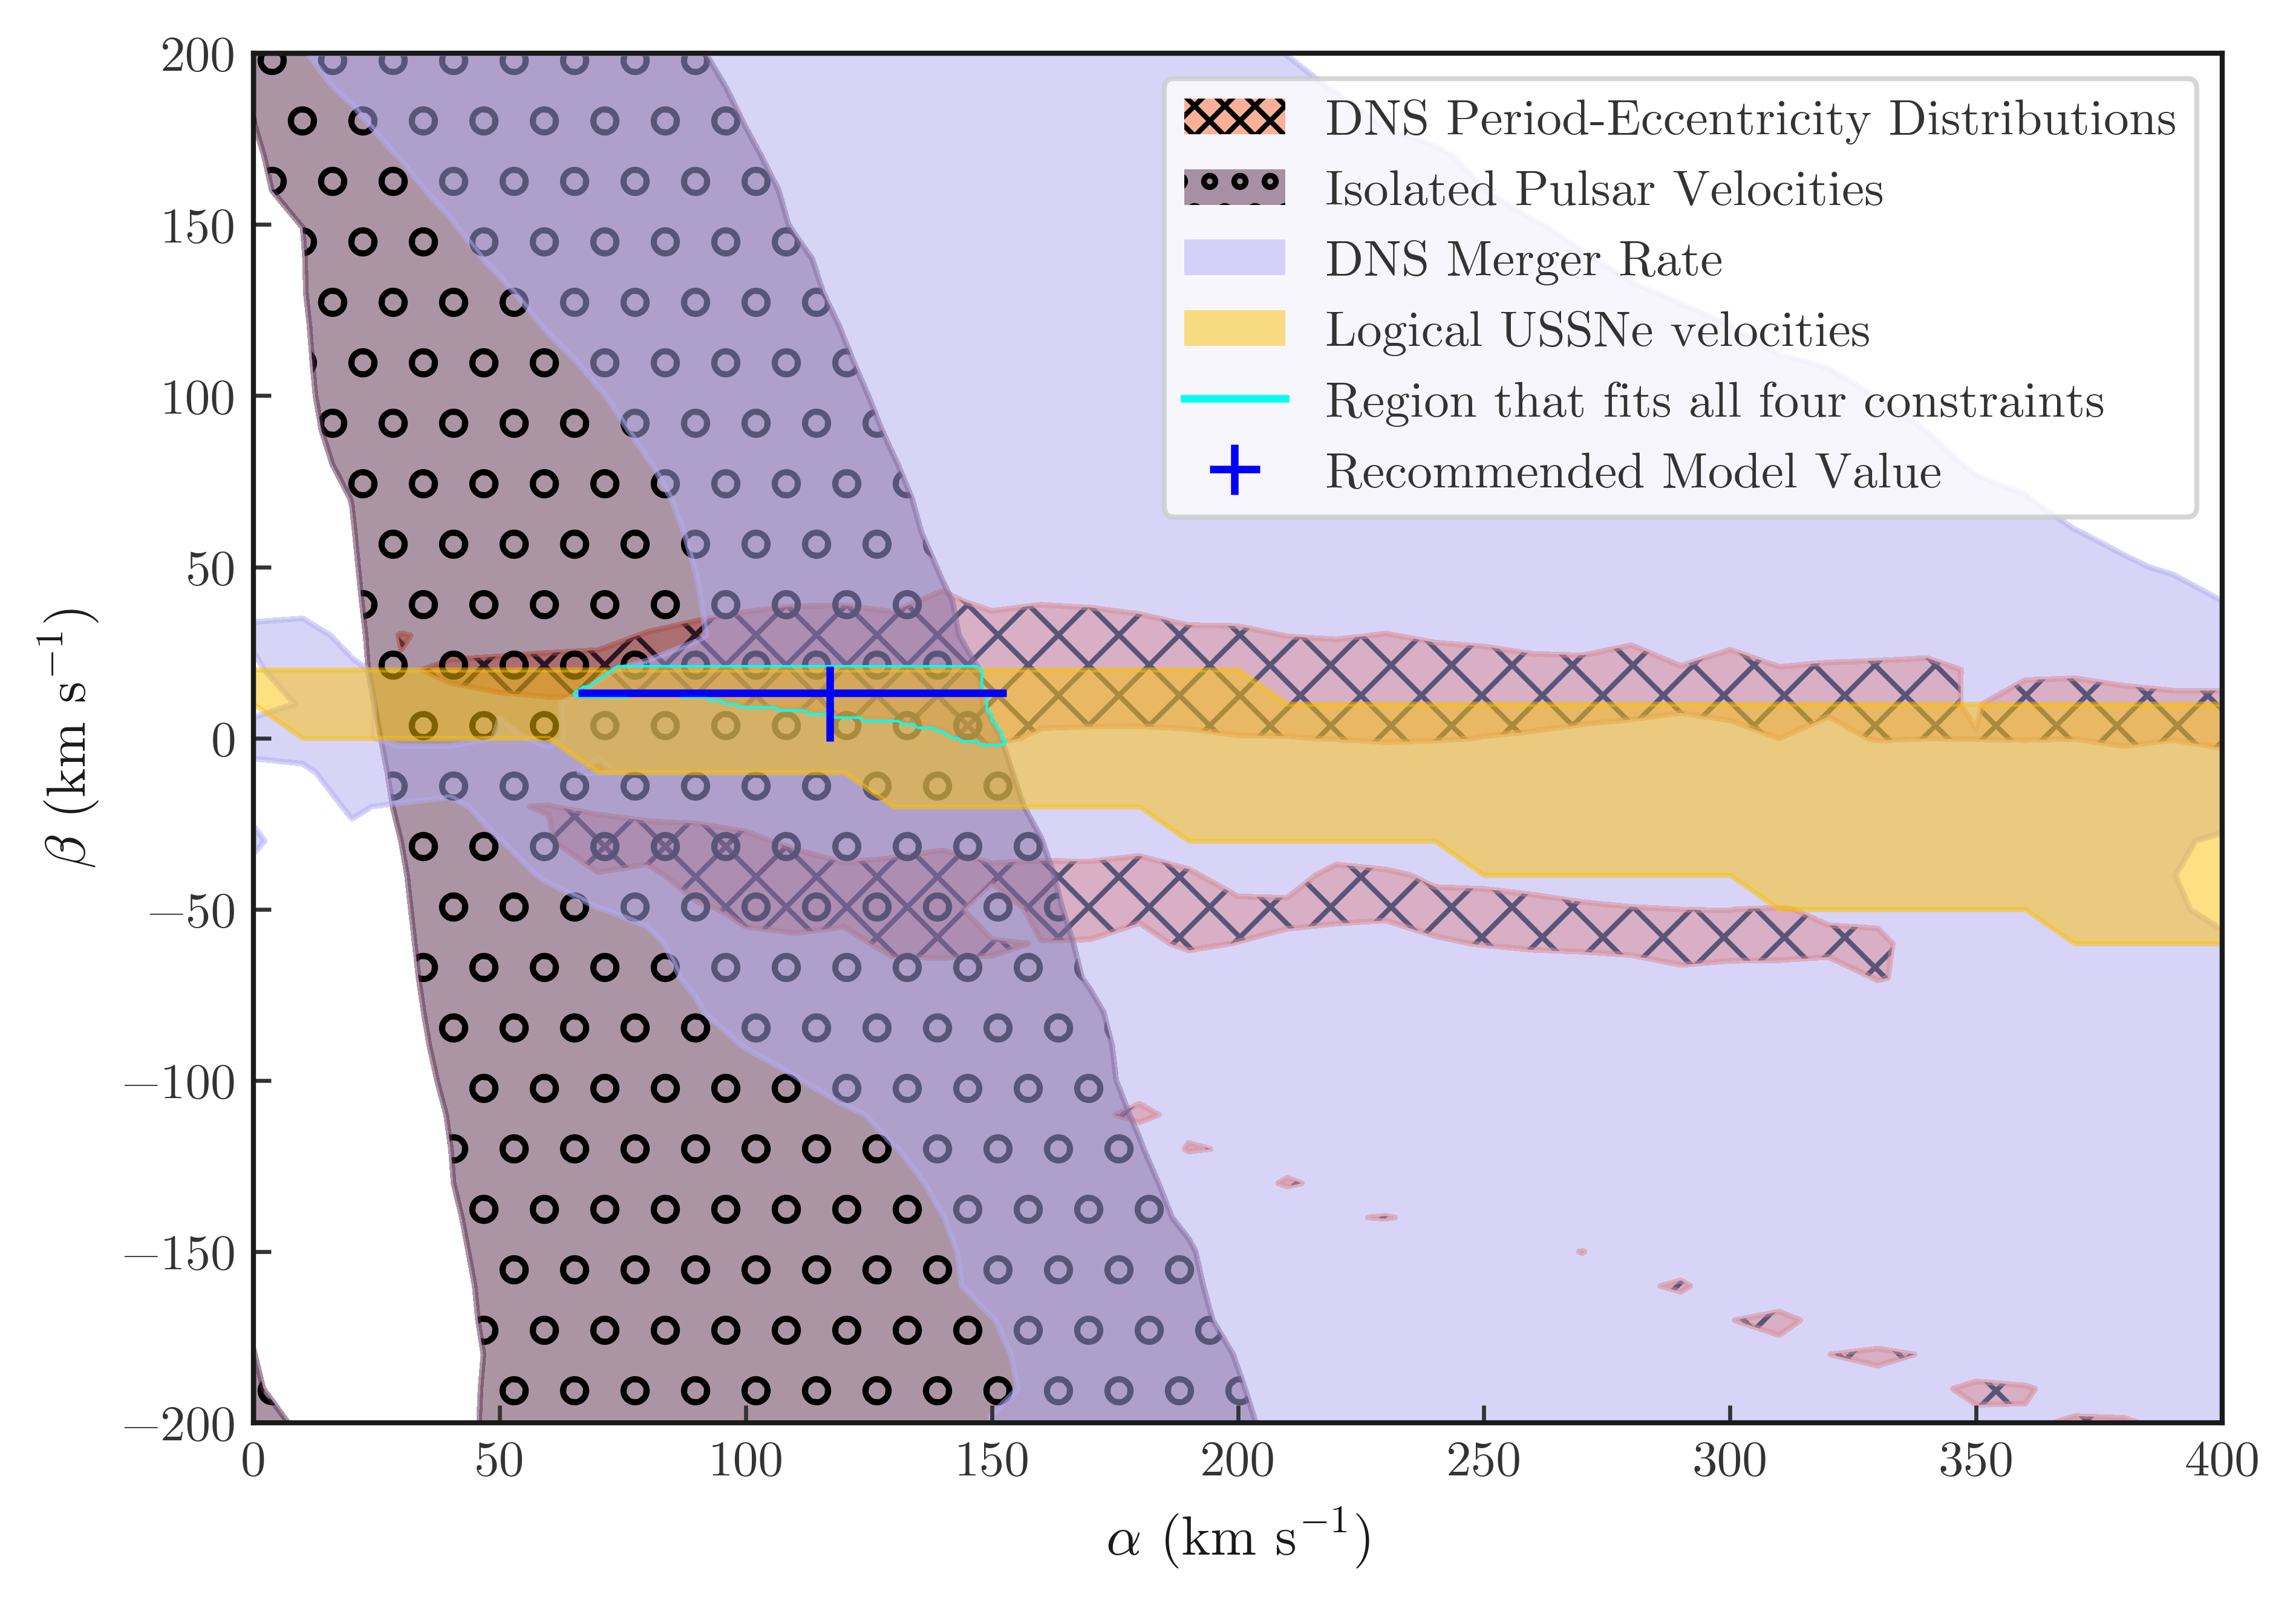
\includegraphics[width=\textwidth]{images/NatalKicks/All_Three_Constraints_with_USSNe_and_modeltype2.png}
    \caption[The four constraints we apply overlaid on our \textsc{FineGrid} parameter space.]{The four constraints we apply overlaid on our \textsc{FineGrid} parameter space. The cyan region represents the region which fits all four parameters, and the blue cross represents the ``center of mass'' of this region.}
    \label{fig:all_four_constraints_on_kicks}
\end{figure}

In \autoref{fig:best_model_params}, we present the two major inferred properties of our recommended model value. First, we present the \glspl{cdf} of a population governed by a Bray kick with the recommended parameters, contrasted with the associated Hobbs kick and observed \citet{Willcox:2021} data. We also show the period-eccentricity distribution of the population, with the observed systems from \autoref{tab:observed_BNSes} overlaid atop the distribution.

\begin{figure}[!htbp]
    \centering
    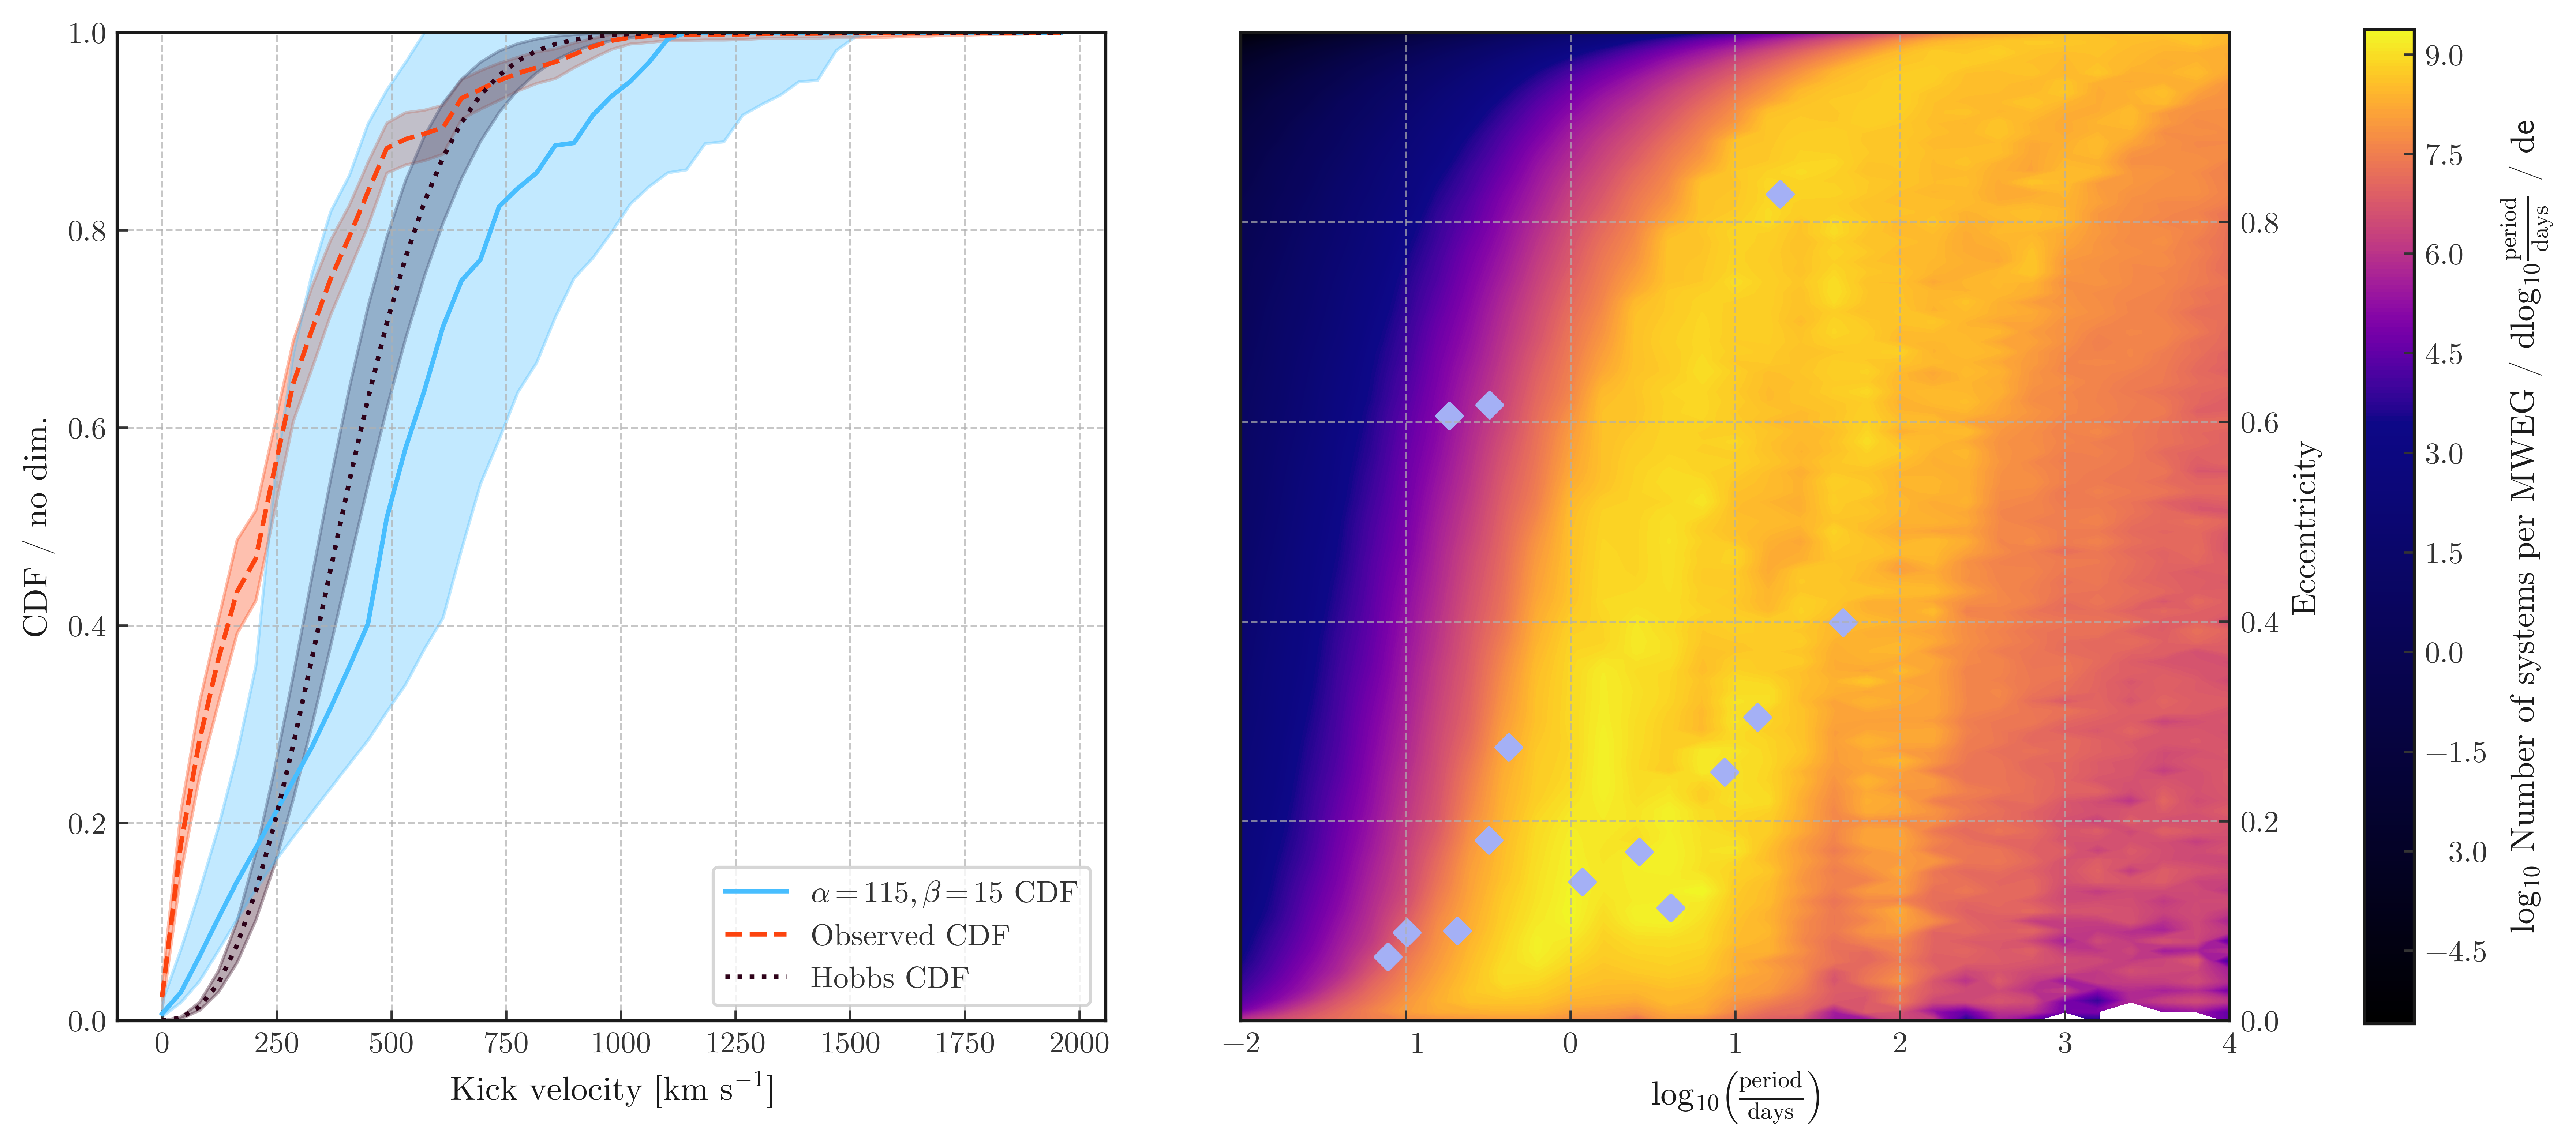
\includegraphics[width=\textwidth]{images/NatalKicks/Best_Model_Params.png}
    \caption[The \acrshort{cdf} for a population of isolated pulsars and the period-eccentricity distribution for $\alpha=\SI{115}{\km\per\s}, \beta=\SI{15}{\km\per\s}$.]{The \gls{cdf} for a population of isolated pulsars (left) and the period-eccentricity distribution (right) for $\alpha=\SI{115}{\km\per\s}, \beta=\SI{15}{\km\per\s}$. The blue region on the \gls{cdf} plot shows the uncertainty region for the reported value. The red region shows the uncertainty band on the \citet{Willcox:2021} \gls{cdf}, which was computed by sampling the \gls{pdf} 10,000 times, taking 2,000 samples each time, and plotting the extent of the simulated distribution. The black band is the uncertainty on the Hobbs distribution, taking $\sigma_\text{max}=\SI{291}{\km\per\s}$ and $\sigma_\text{min}=\SI{239}{\km\per\s}$ from \citet{Verbunt:2017}.}
    \label{fig:best_model_params}
\end{figure}

We are also able to extrapolate this to comment on the expected peak of the event-rate distribution. Given that the event rate is a convolution between the merger rate of our population and the \gls{sfrd} we choose (cf. \autoref{eq:event_rate_distribution}), by affixing the \gls{sfrd} across our populations, by \autoref{eq:definition_of_merger_rate} we can vary $\mathcal{R}(t)$ by varying $\alpha$ and $\beta$. Since the \gls{sfrd} is of a Gaussian form (with a peak at $z\sim1.863$), we can also extract the peak of the distribution assuming it is governed by a particular $\alpha$-$\beta$ combination. The general results across the parameter space are shown in \autoref{fig:grid_shifting_peak}. The best model choice parameters we find fall within the valley of $z=0$, indicating that the peak of the event rate distribution is the present day.

We note that there is a single peak at $\alpha=\SI{330}{\km\per\s}, \beta=\SI{-70}{\km\per\s}$ which appears to be an outlier when compared to its neighbours. We display in \autoref{fig:grid_shifting_peak_zoomed} the local behaviour of the 9 cells around this region. One can see that this beak is bimodal with a second peak at $z=0$, which is only 0.098 per cent lower than the reported peak, clearly resulting in a simple outlier.

\begin{figure}[!htbp]
    \centering
    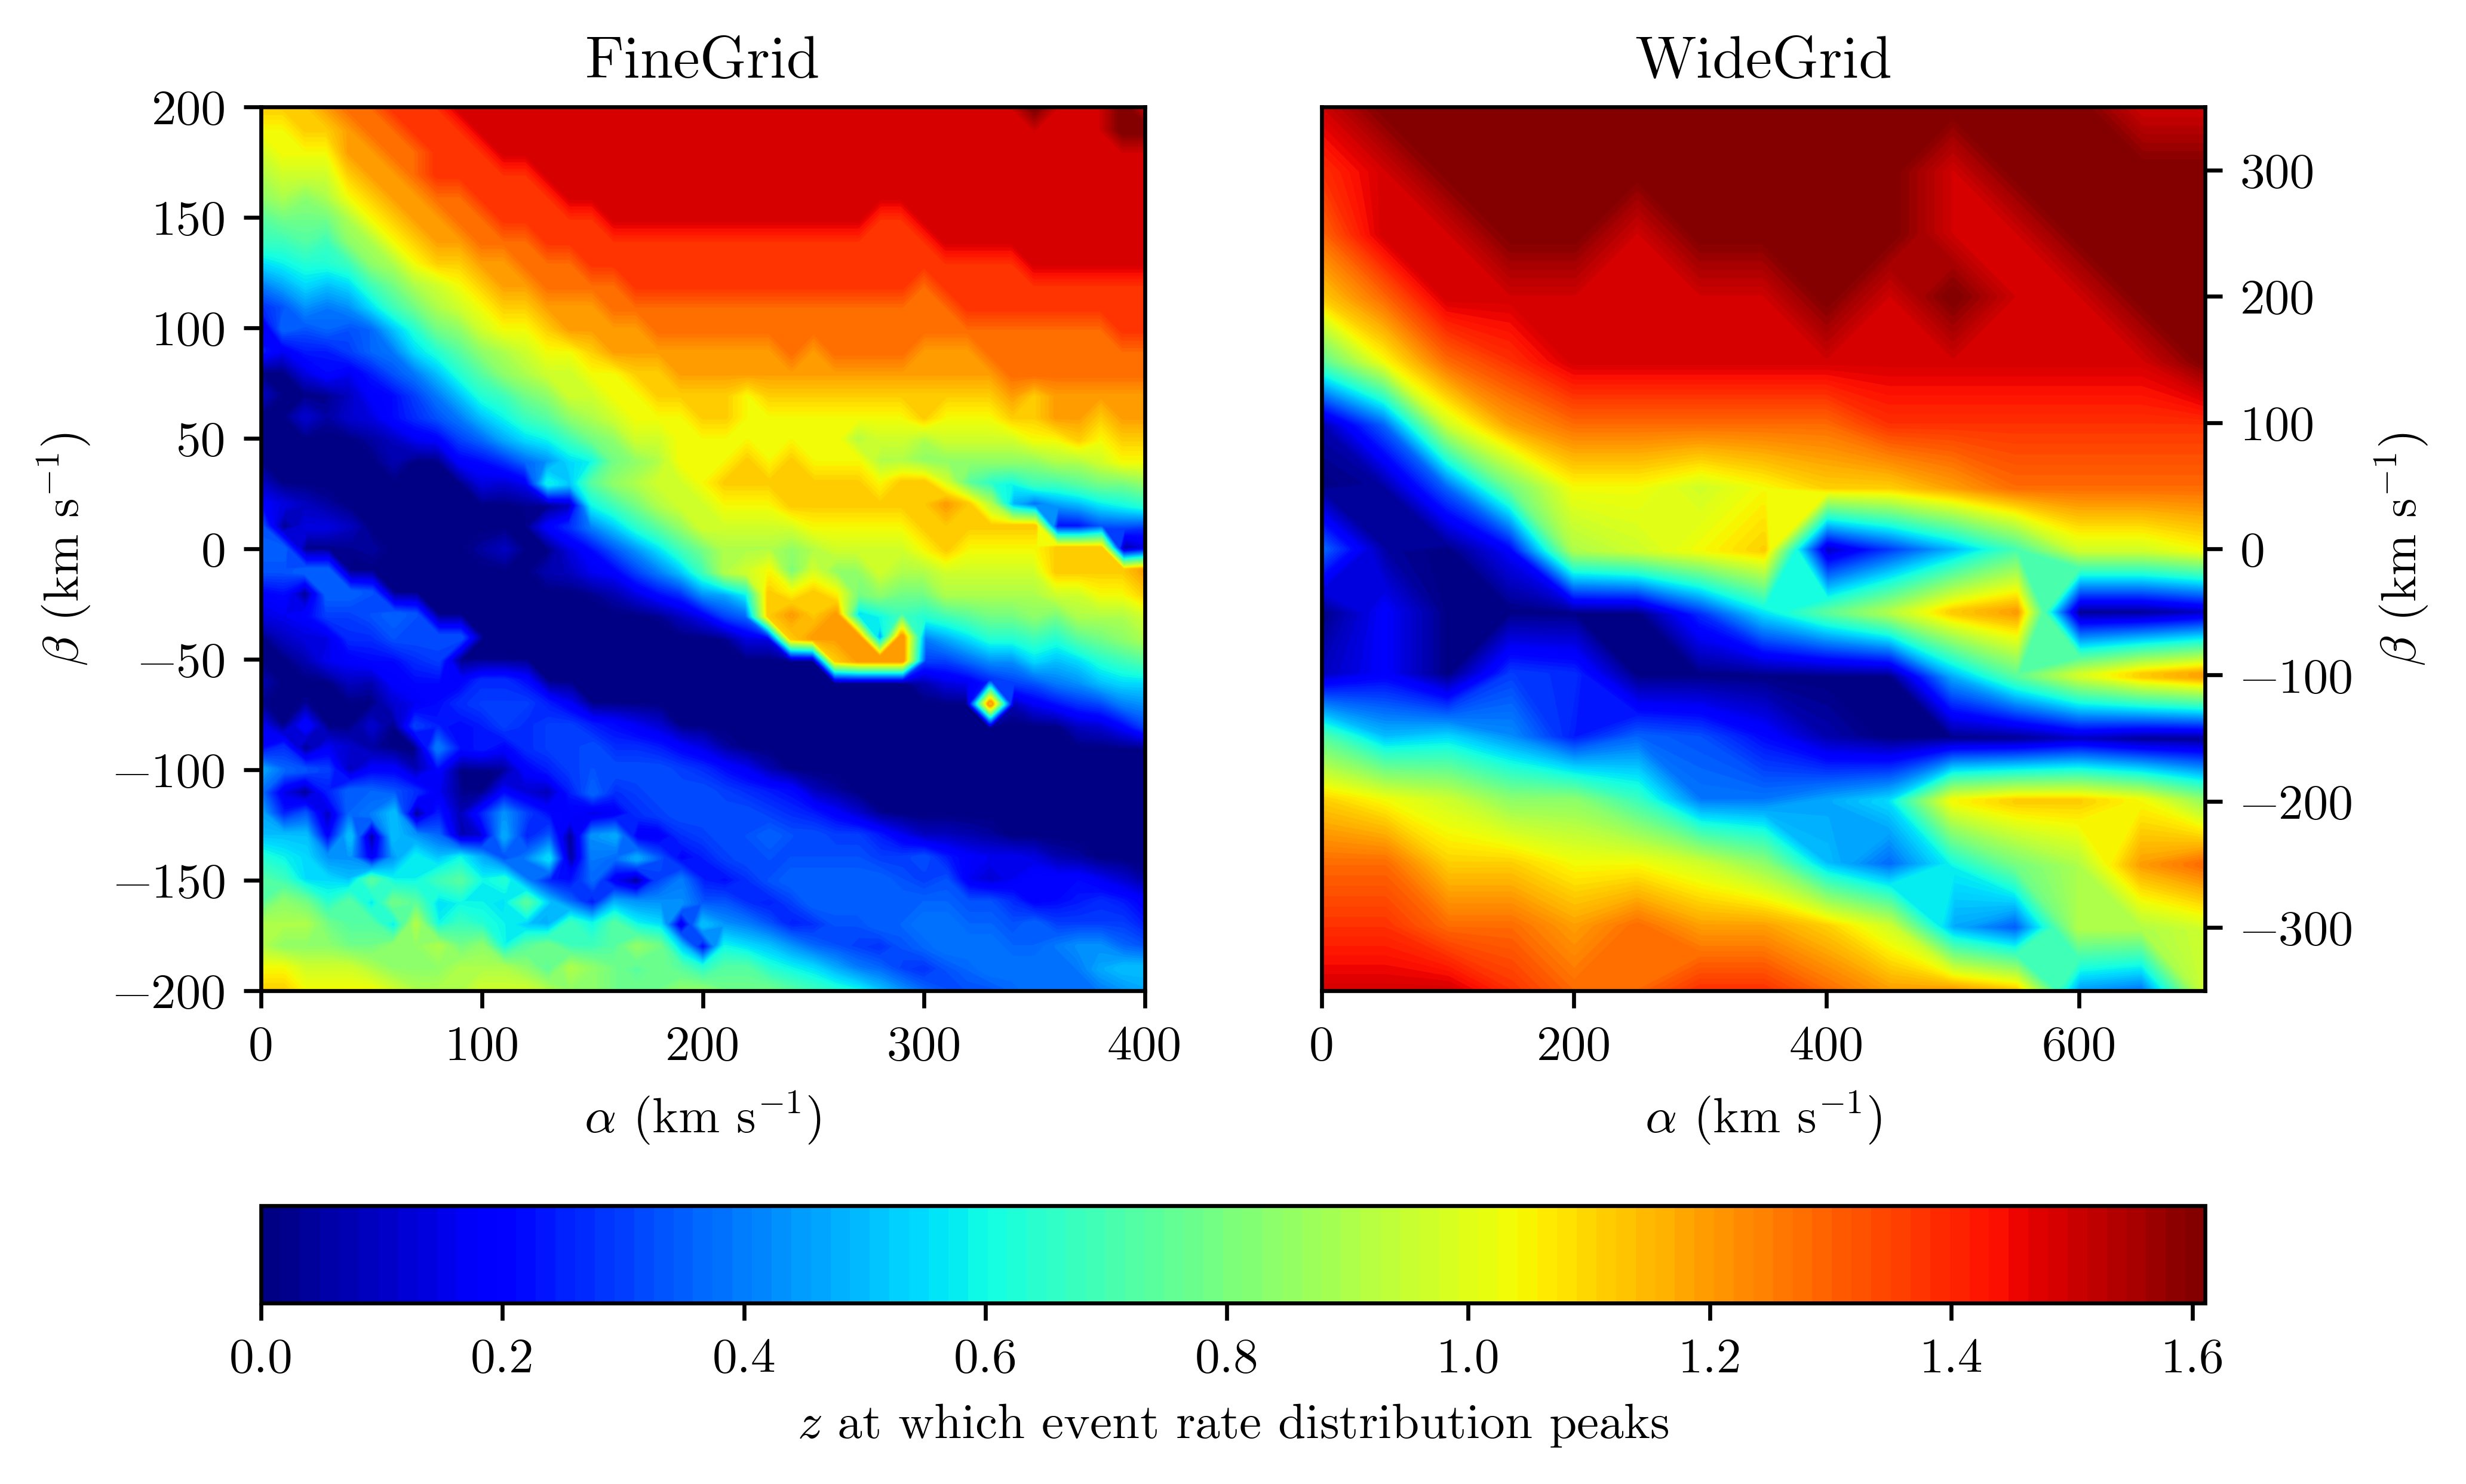
\includegraphics[width=\textwidth]{images/NatalKicks/grid_shifting_peaks.png}
    \caption[The peak of the event rate $\mathcal{R}(t)$ as a function of $\alpha$ and $\beta$.]{The peak of the event rate $\mathcal{R}(t)$ as a function of $\alpha$ and $\beta$. Varying these two parameters generally brings the peak closer to the present day ($z=0$). Absent a merger rate (or, more formally, assuming the merger rate is instantaneous and given by a Dirac-delta function), the \gls{sfrd} peaks at $z\sim1.863$. The region surrounding the peak at $\alpha=330, \beta=-70$ is shown in \autoref{fig:grid_shifting_peak_zoomed}.}
    \label{fig:grid_shifting_peak}
\end{figure}

\begin{figure}[!htbp]
    \centering
    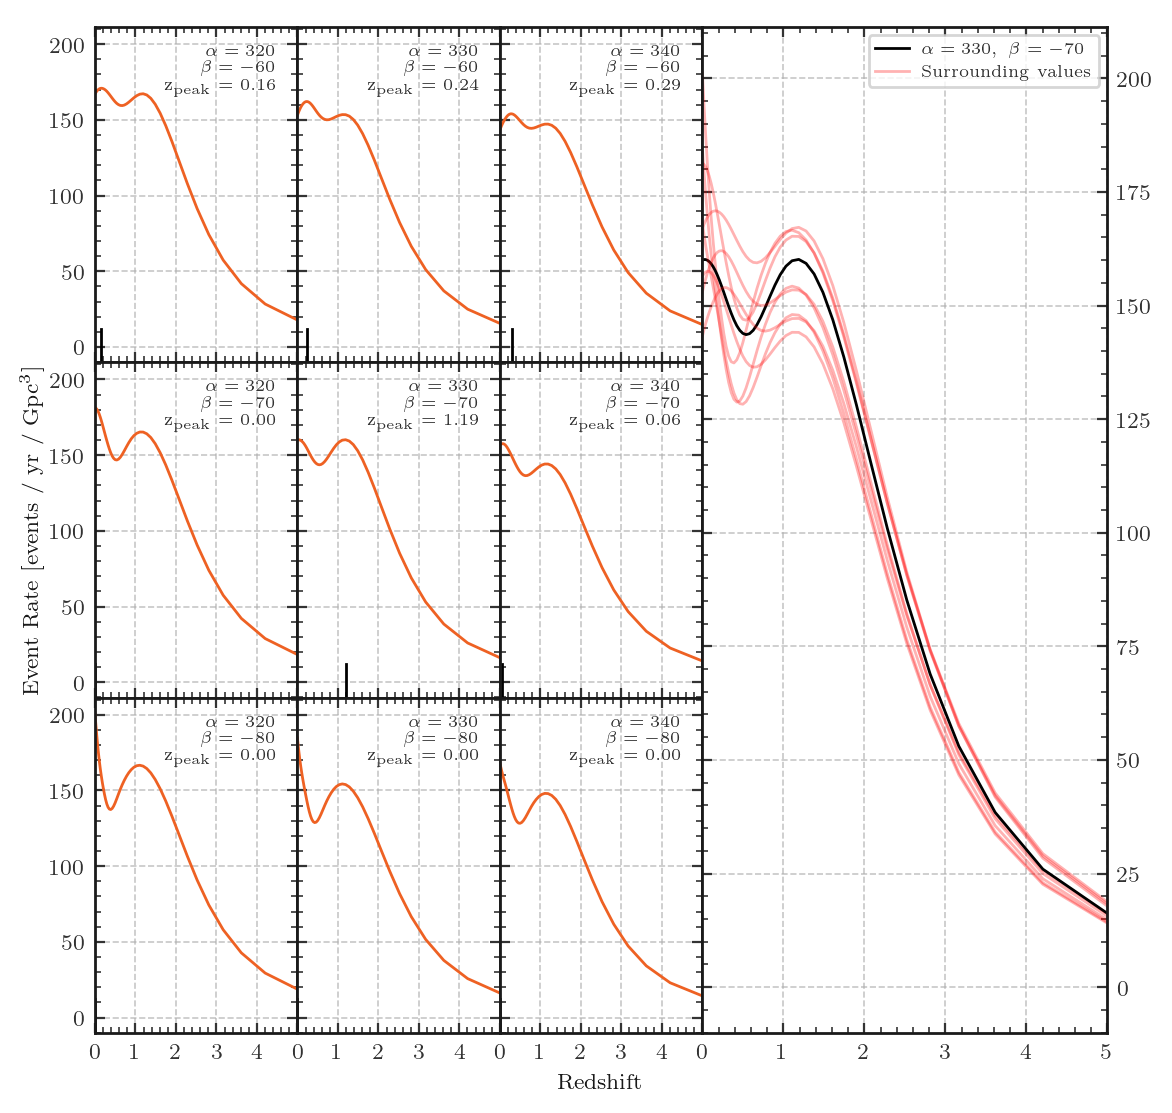
\includegraphics[width=\textwidth]{images/NatalKicks/event_rate_history_local.png}
    \caption[The event rate $\mathcal{R}(z)$ for a region surrounding $\alpha=330, \beta=-70$ on \textsc{FineGrid}.]{The event rate $\mathcal{R}(z)$ for a region surrounding $\alpha=330, \beta=-70$ on \textsc{FineGrid}. This region corresponds to the ``outlier'' in \autoref{fig:grid_shifting_peak}. Shown on the left are the outlier bin in the center and its neighbours in both $\alpha$-space and $\beta$-space. The black line on each plot denotes the location in redshift of the event rate distribution peak. The right plot shows the outlier in black and its neighbours in faded red behind.}
    \label{fig:grid_shifting_peak_zoomed}
\end{figure}

Unfortunately, there is a paucity of observational evidence to confirm whether or not the peak is truly the present day. Given that a redshift of $z=2$ corresponds to a lookback time of $t_\text{LB}=\SI{10}{\giga\year}$, we lack evidence to corroborate this prediction. The next generation of telescopes, including \gls{jwst}, may yet be able to constrain this result further. In the interim, indirect evidence may be able to be applied via the r-process enrichment history of the Milky Way. \citet{Van_de_voort:2022}, for example, finds that greater velocity natal kicks would be correlated with fewer r-process enhanced stars in the Milky Way, as higher kicks would unbind more binaries, meaning that r-process elements are no longer able to accrete onto star-forming regions. \citet{Kobayashi:2023} indicates that current population synthesis models\footnote{Explicitly considered in the paper are COMPAS \citep{Team_compas_riley:2022}, StarTrack \citep{Belczynski:2020}, Brussels \citep{Mennekens:2014, Mennekens:2016}, ComBinE \citep{Kruckow:2018}, and BPASS \citep{Eldridge:2017}.} are unable to reproduce the abundance distributions of certain high-mass isotopes, including the abundances of Oxygen, Iron, Europium, Gold, and Uranium.

\section{Discussion}

There are limitations to this analysis. The first is that we did not preferentially weight our binaries. \citet{Tauris:2017} for example places particular weight on PSR J1930-1852, which is a particularly wide binary. Per \citet{Swiggum:2015} (who reported it), ``its unique spin and orbital parameters challenge models that describe BNS formation'', which implies that any credible model of \gls{bns} formation should replicate its orbital parameters. We did find in \autoref{fig:o3a_contour_figure} that some parameters had non-zero probability of replicating this pulsar, which indicates that the Bray kick is able to reproduce it.

Secondly, we have assumed Newtonian mechanics. Formally, the derivations presented earlier (cf. \autoref{sec:binary_kinematics}) assumed general relativity for the existence of the gravitational wave equation,\footnote{Here, $\tensor{\bar{h}}{_{\mu\nu}}$ is the trace inverse of a weak perturbation to locally Minkowski spacetime with positive-definite trace, and $\Box$ is the d'Alembertian operator.}

\begin{equation}
    \Box \tensor{\bar{h}}{_{\mu\nu}} = -\frac12 \sqrt{32\pi G}\tensor{T}{_{\mu\nu}},\label{eq:GW_spacetime_equation}
\end{equation}

but the injected physics was Newtonian (see \citet{Richards:2021} for a derivation). Strictly speaking, relativistic corrections apply to these kinematic equations too. The logic outlined in \autoref{sec:relativity_exists} ceases to apply, as we are not modelling the interior of a star. Instead, one would need to apply corrections to the two-body equation of motion, termed the post-Newtonian approximation. The general equation becomes

\begin{equation}
    \dv{\vec{v}}{t} = \frac{G\left(m_1+m_2\right)}{r^2}\left(-\hat{n} + \sum_{k=2}^N \frac{1}{c^k}\vec{A}_{\frac{k}{2}\text{PN}} \right),
\end{equation}

where $N$ is the highest order term considered, and $\vec{A}_{\frac{k}{2}\text{PN}}$ is termed the ``$\frac{k}{2}$-th Post-Newtonian'' coefficient. Testing with the \codename{riroriro} code from \citet{Van_zeist:2021} indicated that including terms up to $N=6$ (3PN) increases the merger time by fractions of a year, and thus does not significantly alter the merger rate density we observe.  Typically 3.5PN ($N=7$) is used as an upper bound \citep{Itoh:2003}, though up to 10PN ($N=20$) has been used before \citep[][and references therein]{Blanchet:2014}.

Relativistic corrections also typically manifest in using more sophisticated spacetime metrics. \autoref{eq:GW_spacetime_equation} assumes a metric which is locally Minkowski, that is

\begin{equation}
    \tensor{g}{_{\mu\nu}} = \tensor{\eta}{_{\mu\nu}}+\sqrt{32\pi G} \tensor{h}{_{\mu\nu}},
\end{equation}

where $\tensor{\eta}{_{\mu\nu}}$ is the positive-definite Minkowski metric. This ``weak-field'' approximation breaks down when a compact object enters within its companion's \gls{isco}, given by $r_\text{isco}=\frac{6GM}{c^2}$, where matter can be exchanged. Given gravitational waves result in strains on the order of $10^{-19}$ \citep{Van_zeist:2023}, representing observed fractional shifts on Earth smaller than the diameter of a proton, \citep{Moore:2014}, the weak field regime suits, and again modelling the relativistic corrections to the post-\gls{isco} regime only increases the merger rate by fractions of years.

To contextualise this case study, other authors such as \citet{Mapelli:2018, Wiktorowicz:2019, Giacobbo:2020, Santoliquido:2021, Kapil:2023} have explored the parameter space of \gls{bns} kicks, though none have performed the analysis in the way we have. These works typically vary the progenitor population properties, in such a way that the formed binaries can in principle vary strongly. However, in our population synthesis procedure, we are able to effectively affix the physics between different models such that \textit{only} the kick velocities are expected to vary between individual populations. Since the Bray kick has two parameters which can be altered, we are able to modify the kick velocity without changing the physics, thus allowing us to isolate and study the kick mechanism alone.

\section{Chapter Summary}

We have presented a formalism for evaluating and quantifying the goodness-of-fit of the natal kick mechanism against four independent tests. The tests we have presented -- constraining the merger rate of \gls{bns} systems, the period-eccentricity distribution of Galactic \gls{bns} systems, the kick velocities of single-star pulsars, and the production of \acrlongpl{ussne} -- greatly constrain the parameter space to be less than 1 per cent of the possible parameters. Furthermore, the data suggest that the peak of the merger rate distribution is the present day, with $z\simeq 1.5$ as the upper bound of the entire parameter space, and $z=0$ for our recommended value.
